%%%%%%%%%%%%%%%%%%%%%%%%%%%%% Define Article %%%%%%%%%%%%%%%%%%%%%%%%%%%%%%%%%%
\documentclass{article}


%%%%%%%%%%%%%%%%%%%%%%%%%%%%% Using Packages %%%%%%%%%%%%%%%%%%%%%%%%%%%%%%%%%%
\usepackage{geometry}
\usepackage{pgfplots}
\usepackage{lipsum}
\usepackage{mdframed}
\usepackage{amsthm}
\usepackage{bm}
\usepackage{titlesec}
\usepackage{tocloft}
\usepackage{ragged2e}
\usepackage{fancyhdr}
\usepackage{glossaries}
\usepackage[spanish]{babel}
\usepackage[sorting=none]{biblatex}
\usepackage[hidelinks]{hyperref}
\usepackage[all]{hypcap}
\usepackage{csquotes}
\usepackage{pdfpages}
\usepackage{booktabs,multirow}
\usepackage{listings}
\usepackage{dirtree}


%%%%%%%%%%%%%%%%%%%%%%%%%% Page Setting %%%%%%%%%%%%%%%%%%%%%%%%%%%%%%%%%%%%%%%
\geometry{a4paper}
\graphicspath{{img/}}
\addbibresource{bibliography.bib}
\numberwithin{figure}{section}
\numberwithin{table}{section}
\setlength{\belowcaptionskip}{5pt} 

\titleformat{\paragraph}
{\normalfont\normalsize\bfseries}{\theparagraph}{1em}{}
\titlespacing*{\paragraph}
{0pt}{3.25ex plus 1ex minus .2ex}{1.5ex plus .2ex}

\fancyhf{}
\pagestyle{fancy}
\fancypagestyle{plain}{}
\lfoot{\thepage}
\fancyhead{}
\renewcommand{\headrulewidth}{0pt}

\lhead{PROYECTO FIN DE GRADO}

\titleformat{\section}
{\rmfamily\Large\raggedleft\uppercase}{\thesection.}{0.1cm}{}[{\titlerule[0.5pt]}]
\titleformat{\subsection}
    {\rmfamily\large\uppercase}{\thesubsection.}{0.1cm}{}

%%%%%%%%%%%%%%%%%%%%%%%%%%%%%%% Plotting Settings %%%%%%%%%%%%%%%%%%%%%%%%%%%%%
\usepgfplotslibrary{colorbrewer}
\pgfplotsset{width=8cm,compat=1.9}


%%%%%%%%%%%%%%%%%%%%%%%%%%%%%%% Title & Author %%%%%%%%%%%%%%%%%%%%%%%%%%%%%%%%
\title{Redes Neuronales Convolucionales}
\author{Asier Villar}


%%%%%%%%%%%%%%%%%%%%%%%%%%%%%%% Components %%%%%%%%%%%%%%%%%%%%%%%%%%%%%%%%%%%
\newcommand{\listequationsname}{\Large{Índice de ecuaciones}}
\newcommand{\myequations}[1]{
    \addcontentsline{equ}{myequations}{\protect\numberline{\theequation}#1}
}

\newcommand{\equationNote}[2]{
    \begin{align} \label{#2} \ensuremath{#1} \end{align} 
    \myequations{#2} \centering \small \textit{#2} \normalsize \justify 
}

\newlistof{myequations}{equ}{\listequationsname}
\setlength{\cftmyequationsnumwidth}{2.3em}
\setlength{\cftmyequationsindent}{1.5em}


%%%%%%%%%%%%%%%%%%%%%%%%%%%%%%% Document %%%%%%%%%%%%%%%%%%%%%%%%%%%%%%%%%%%%%
\begin{document}

    \pagenumbering{roman}
    
\includepdf[pages={1}]{frontpage.pdf}
    
\includepdf[pages={1}]{frontpage.pdf}
    \section*{Resumen}
El propósito del siguiente proyecto es investigar y desarrollar una nueva solución para el 
problema de optimización “flexible job shop scheduling problem” (FJSP), que se clasifica dentro 
de la categoría de problemas NP-hard, que son aquellos que no pueden ser resultados de forma 
exacta por un algoritmo en un tiempo de computación polinómica. El objetivo es asignar una 
serie de operaciones a un conjunto de máquinas, teniendo en cuenta una lista de restricciones 
y requisitos, como por ejemplo el tiempo de procesamiento. Por último, como resultado de lo 
anterior, se proveerá de una configuración válida, que intente minimizar el tiempo máximo de 
finalización (make span) de todas las máquinas.\medskip 

Se propone utilizar técnicas de Imitation Learning, una variante del Reinforcement learning 
que permite al modelo aprender a partir de ejemplos proporcionados por un experto. En nuestro 
caso, se estudiarán técnicas de generación de ejemplos válidos que permitan al modelo aprender 
técnicas para resolver el FJSP. La idea, es extraer configuraciones óptimas de instancias 
pequeñas generadas aleatoriamente y utilizarlas como datos de entrenamiento para un modelo, 
que pueda desarrollar una estrategia propia en base a las decisiones del experto y posteriormente 
generalizar a instancias mayores.\medskip 

El objetivo es mejorar la velocidad en la que se ofrecen planificaciones cercanas al óptimo, 
ya que con este planteamiento no será necesario explorar todo el espacio de soluciones. Otro 
de los beneficios es la adaptabilidad a variaciones del problema dinámicamente, como cambios 
en los tiempos de procesamiento o la incorporación de nuevas operaciones. Teniendo esto en 
cuenta, se espera obtener una solución en tiempo lineal que no se desvíe excesivamente del 
óptimo y que pueda aplicarse a diferentes escenarios industriales e incluso en consonancia 
con otras técnicas.

\section*{Descriptores}
Reinforcement Learning, Imitation Learning, FJSP, Redes Neuronales, MLOPS
\pagebreak 
    \tableofcontents
\listoftables
\listoffigures
\pagebreak 
 

    \pagenumbering{arabic}
    \section{Introducción}
La planificación de la producción es una disciplina clave en la gestión de 
activos y se utiliza para determinar la forma más eficiente de asignar 
recursos, como maquinaria, mano de obra y tiempo, con el fin de alcanzar 
los objetivos de producción. Es un proceso que implica la toma de decisiones 
sobre qué recursos, cuánto, cuándo y cómo producirlos, con el objetivo de optimizar la 
utilización de los elementos disponibles, maximizando la eficiencia y rentabilidad 
del proceso de producción. La planificación de la producción se aplica en una 
amplia gama de sectores y áreas de negocio, incluyendo la fabricación, la logística, 
el transporte, la distribución y la gestión de la cadena de suministro, entre otros.\medskip

La importancia de la planificación de la producción radica en su capacidad para mejorar 
la eficiencia mediante una buena gestión de las operaciones, lo que puede tener un impacto 
significativo en la rentabilidad y competitividad de las empresas. Una planificación de 
producción efectiva debe optimizar la asignación de recursos, minimizar los tiempos de 
inactividad, reducir los costos de producción y maximizar el cumplimiento de los plazos 
de entrega en la medida de lo posible. Esto lo que resulta es en una mayor eficiencia operativa 
y una mejor calidad del producto o servicio.\medskip

Sin embargo, la planificación de la producción es un problema complejo debido a la gran 
cantidad de variables y restricciones que deben tenerse en cuenta, como los tiempos de 
procesamiento, las capacidades de los recursos, las restricciones de almacenamiento y 
transporte y las demandas de los clientes, entre otros. Tradicionalmente, este problema 
se ha abordado utilizando enfoques heurísticos y algoritmos de optimización, como el 
Job Shop Scheduling Problem (JSP) y el Flexible Shop Scheduling Problem (FJSP), que son problemas 
combinatorios y conocidos por ser NP-Hard, lo que implica que no existen algoritmos eficientes 
para encontrar soluciones óptimas en un tiempo razonable.\medskip

Un problema NP-Hard es un tipo de problema de optimización en el cual no se conocen algoritmos 
eficientes que puedan encontrar una solución óptima en un tiempo polinómico. Esto implica que a 
medida que el tamaño del problema aumenta, el tiempo de cómputo necesario para encontrar una 
solución óptima también se vuelve prohibitivamente alto. Estos problemas son considerados de 
gran complejidad y representan un desafío significativo para la investigación en ciencias de 
la computación. La importancia de identificar un problema como NP-Hard radica en que a menudo 
tecnicas utilizadas para un problema pueden ser aplicados a otros problemas NP-Hard. Esto se debe a que 
muchos problemas NP-Hard comparten estructuras y patrones similares, lo que permite la 
transferencia de conocimientos y técnicas de un problema a otro. Por lo tanto, encontrar 
soluciones eficientes o aproximadas para un problema NP-Hard particular puede tener un impacto 
significativo en la resolución de otros problemas que enfrentan desafíos similares\medskip

En los últimos años, ha surgido el Imitation Learning como una prometedora técnica de aprendizaje 
automático. El Imitation Learning se basa en el concepto de aprender de la experiencia de expertos 
humanos o de sistemas de planificación previamente establecidos, y luego utilizar ese conocimiento para 
guiar la toma de decisiones en situaciones similares. Esto se puede lograr a través de enfoques 
supervisados, donde se entrena a un modelo para imitar las acciones de expertos humanos, o 
a través de enfoques de Reinforcement Learning (RL), donde se permite que un modelo aprenda a 
partir de la retroalimentación y la interacción con el entorno.\medskip

En este contexto, el presente trabajo se enfoca en el desarrollo de un sistema de planificación 
de la producción basado en Imitation Learning, utilizando técnicas de aprendizaje supervisado y RL. 
Se busca explorar cómo estas técnicas pueden aplicarse a la planificación de la producción, teniendo 
en cuenta los desafíos y la complejidad de este problema. A través del estudio y análisis de 
diferentes enfoques y metodologías, se pretende contribuir al campo de la planificación de la 
producción utilizando técnicas de inteligencia artificial y aprendizaje automático, con el objetivo 
de mejorar la eficiencia y la toma de decisiones en procesos industriales.\medskip

\subsection{Motivación}
La planificación de la producción es un desafío constante en la industria, ya que puede tener 
un impacto significativo en la eficiencia, la productividad y la rentabilidad de las operaciones 
de fabricación. Sin embargo, muchos de los problemas de planificación de la producción en la 
industria, como el Job Shop Scheduling Problem (JSP) y el Flexible Job Shop Scheduling Problem (FJSP), 
son conocidos por su alta complejidad y la falta de soluciones eficientes. Esto puede resultar 
en cuellos de botella, retrasos en la producción y costos innecesarios.\medskip

Es crucial encontrar soluciones innovadoras y eficientes que puedan abordar 
los desafíos complejos asociados con la planificación de la producción en entornos que enfrentan 
problemas NP-Hard. Además, la aplicación de enfoques de inteligencia artificial y aprendizaje 
automático en la planificación de la producción ha ganado cada vez más atención en la industria 
debido a su potencial para encontrar soluciones aproximadas en tiempo real y adaptarse a 
entornos dinámicos.\medskip

La motivación de este proyecto radica en la necesidad de desarrollar enfoques de Imitation 
Learning, una rama del aprendizaje automático que se basa en la imitación de comportamientos 
de expertos, para abordar los desafíos de la planificación de la producción en la industria. 
Estos enfoques tienen el potencial de mejorar la eficiencia y la productividad de las operaciones 
de fabricación al encontrar soluciones eficientes y adaptativas en tiempo real. Además, las 
soluciones desarrolladas en el contexto del JSP y el FJSP podrían tener aplicaciones amplias 
en otros problemas NP-Hard que enfrenta la industria, como la logística, la programación de 
tareas o la asignación de recursos, lo que podría tener un impacto significativo en la 
optimización de procesos y la competitividad de las empresas en la industria.

\subsection{Explicación del problema}
El Flexible job shop scheduling problem (FJSP), es un desafío de optimización combinatoria 
que se encuentra en el campo de la la gestión de la producción. En este problema, se busca determinar 
la secuencia óptima de operaciones a realizar en una serie de máquinas, con el objetivo de minimizar el 
tiempo total de producción o maximizar la eficiencia del sistema. A diferencia del Job shop scheduling 
problem (JSP), en el que cada operación tiene una ruta de procesamiento fija, las operaciones pueden ser 
procesadas en varias máquinas diferentes. Además, adicionalmente las operaciones estan agrupadas 
dentro de un trabajo, que es un conjunto de operaciones que deben ser procesadas en una secuencia
específica.\medskip

Existen dos restricción temporales que especifican cuándo puede comenzar 
cada operación: una operación no puede comenzar hasta que se hayan completado todas las operaciones
anteriores de la misma tarea y no puede comenzar hasta que se hayan completado todas las operaciones
anteriores de la misma máquina. El objetivo del problema es asignar las operaciones a las máquinas y determinar el orden de procesamiento 
del sistema manera óptima, teniendo en cuenta las restricciones temporales y los recursos disponibles, 
de manera que se minimice el tiempo total de producción. El tiempo total de producción se refiere al
tiempo de finalización de la máquina más lenta, que se calcula sumando el tiempo de procesamiento 
de todas las operaciones y el gap que estas generan.\medskip

Para ilustrar el problema, supongamos que tenemos una fabrica que produce tres tipos de productos
que se definen como los trabajos: A, B y C. Contamos con tres máquinas: M1, M2, M3 y M4 
y cada producto requiere hacer ciertas operaciones de procesamiento en estas máquinas en 
un orden específico. Las operaciones y los tiempos de procesamiento estimados para cada 
producto en cada máquina son los siguientes: 

\begin{table}[ht]
    \caption{Tiempos de procesamiento estimados para cada producto} 
    \centering 
    \begin{tabular}{ccccccccc}  

    \toprule
    \multirow{2}{*}{\parbox[c]{.2\linewidth}{\centering Maquina ID}} & 
    \multicolumn{2}{c}{Trabajo A} && 
    \multicolumn{2}{c}{Trabajo B} && 
    \multicolumn{2}{c}{Trabajo C} \\ 

    \cmidrule{2-3} \cmidrule{5-6} \cmidrule{8-9}
     & {\centering OP 1} & {OP 2} && {OP 3} & {OP 4} && {OP 5}\\

    \midrule
    Máquina 1 & 4 UT & --   && 3 UT & 7 UT && 1 UT & -- \\
    Máquina 2 & 3 UT & 2 UT && 2 UT & 2 UT && 6 UT & -- \\
    Máquina 3 & 2 UT & 1 UT && --   & 5 UT && 2 UT & -- \\  
    Máquina 4 & --   & 3 UT && 4 UT & 8 UT && 4 UT & -- \\ 
    \bottomrule
    
    \end{tabular}
\end{table}

\medskip

Aquí, cada operación se identifica con un número y el tipo de procesamiento se mide en Unidades temporales
(UD). Las operaciones que no se pueden realizar en una máquina se identifican con un guión (-), lo que 
significa que en este ejemplo la máquina 1 podría procesar las operaciones 1, 3, 4 y 5 pero 
no la operación 2. Una vez entendida la distribución de tiempos de procesamiento, podemos visualizar
el resultado de la planificación en el siguiente diagrama, donde cada caja representa una operación 
y cada línea representa una máquina.

\begin{figure}[ht]
    \centering
    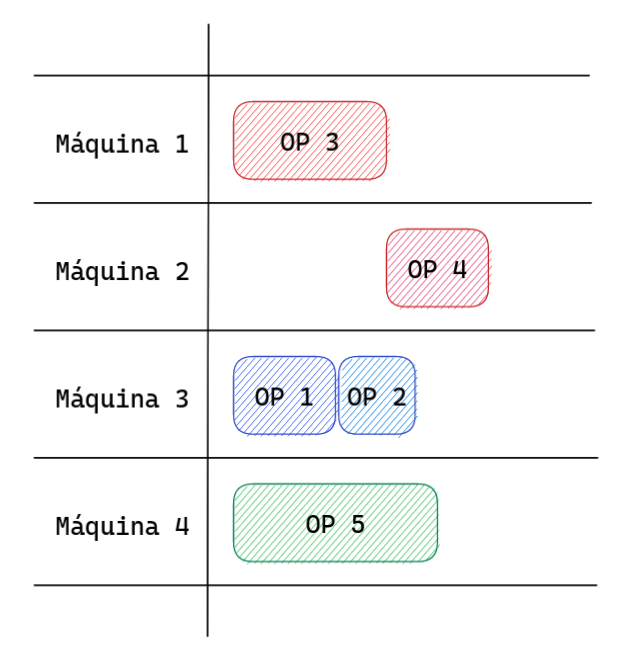
\includegraphics[scale=0.40]{ejemplo.png}
    \caption{Ejemplo de planificación óptima}
    \label{fig:example-solution}
\end{figure}

La distribución final de tiempos para cada máquina es la siguiente: 
\begin{itemize}
    \item \textbf{maquina 1}, OP 3 (3 UT) + 0 GAP = 3 UT 
    \item \textbf{maquina 2}, OP 4 (2 UT) + 3 GAP = 5 UT 
    \item \textbf{maquina 3}, OP 1 (2 UT) + OP 2 (1 UT) + 0 GAP = 3 UT 
    \item \textbf{maquina 4}, OP 5 (4 UT) + 0 GAP = 4 UT. 
\end{itemize}

Ya que el tiempo total de producción es el tiempo de finalización de la máquina más lenta, 
que es la máquina 2, son 5 UT. Notese que el gap de la máquina 2 es deribado de la dependencia
existente entre la operación 4 y la operación 3 por petenercer ambos al trabajo B, 
por lo tanto, antes de que dicha maquina empiece con la operacion 4 tiene que esperar 
a que se procese la máquina 1.

\subsection{Estructura de la memoria}



\pagebreak
    \section{Antecedentes y justificación}
El objetivo de esta seccion es describir las condiciones del entorno en el que se lleva a cabo 
el proyecto, se recopilarán datos e información sobre la situación actual en lo que respecta al FJSP, 
incluyendo la utilización de diferentes tecnicas que han sido utilizadas historicamente para su resolución. 
Para ello, se revisará el estado del arte y las últimas tendencias en este campo, con el fin de obtener una 
mejor comprensión del problema y explicar la oportunidad de realizar nuevos aportes en esta área de investigación.


\subsection{Estado del arte}
\subsubsection{Metodos exactos}
Los métodos exactos se basan en la resolución matemática del problema, y pueden garantizar la 
obtención de soluciones óptimas en teoría. Sin embargo, estos métodos suelen ser computacionalmente 
costosos y, por lo tanto, se aplican principalmente a problemas de tamaño reducido.\medskip

En el caso del FJSP, algunos métodos exactos que se han utilizado incluyen la programación 
lineal de enteros mixta (MILP)\cite{milp}, que modela el problema como un conjunto de restricciones lineales y 
una función objetivo lineal, y la programación por restricciones (CP)\cite{wikiCP}, que reduce el problema a
un conjunto de restricciones lógicas y utiliza técnicas de búsqueda para encontrar soluciones que satisfagan 
todas las restricciones. Existen aplicaciones hechas por google como Ortools\cite{ortools}
o por IBM como CPLEX\cite{cplex}, que son ejemplos de soluciones que utilizan estos métodos exactos para resolver
problemas de optimización. Estas aplicaciones son muy útiles para resolver instancias de tamaño reducido,
pero no son capaces de resolver instancias de tamaño grande, debido a la gigantesca dimensionalidad que
implica el resolver este tipo de problemas por métodos exactos.


\subsubsection{Metodos heurísticos}
Un método heurístico es un algoritmo o técnica de búsqueda que está diseñado para encontrar 
soluciones aproximadas a problemas de optimización, cuando las soluciones exactas son difíciles 
de encontrar. Los métodos heurísticos son útiles cuando el tiempo y los recursos son limitados, 
y cuando el problema a resolver es demasiado complejo para ser resuelto por medios exactos. 
Estos métodos se basan en la experiencia y el conocimiento previo para generar soluciones que 
son buenas pero no necesariamente óptimas. Los métodos heurísticos pueden ser aplicados a una 
amplia variedad de problemas de optimización, incluyendo el FJSP.\medskip

En el caso del FJSP, existen diferentes métodos heurísticos que se han utilizado con éxito 
para encontrar soluciones aproximadas. Un ejemplo es el algoritmo de búsqueda tabú, 
que se basa en la exploración de soluciones vecinas para encontrar soluciones cada vez mejores. 
Otro ejemplo es el algoritmo de búsqueda local, que busca soluciones iterativamente en una 
vecindad de soluciones. También se ha utilizado el enfoque basado en la construcción de 
soluciones parciales, donde se construyen soluciones en etapas, utilizando información previa 
y reglas heurísticas para guiar el proceso de construcción. Todos estos métodos heurísticos 
han demostrado ser efectivos para resolver el problema de FJSP, y se pueden adaptar y mejorar 
para abordar variantes más complejas del problema.

\subsubsection{Algoritmos genéticos}
Los algoritmos genéticos son una técnica de optimización inspirada en la evolución biológica.
Estos algoritmos imitan el proceso de selección natural, reproducción y mutación en la búsqueda 
de soluciones óptimas o cercanas a la óptima para problemas de optimización combinatoria. La 
idea básica de los algoritmos genéticos es utilizar la selección natural para encontrar soluciones
mejores a través de la generación de nuevas soluciones a partir de soluciones existentes y la 
aplicación de operadores de cruce y mutación.\medskip

En la literatura, estos algoritmos han sido ampliamente utilizados y han demostrado ser 
efectivos para encontrar soluciones de alta calidad. La representación cromosómica utilizada 
en los algoritmos genéticos se basa en la codificación de una solución del problema de FJSP 
como una cadena de genes, y los operadores genéticos como el cruzo o la mutación, se aplican 
para producir nuevas soluciones o realizar ligeros cambios en aquellas ya existentes. Una de 
sus principales ventajas es que pueden manejar fácilmente múltiples objetivos y restricciones 
adicionales, y son capaces de explorar ampliamente el espacio de soluciones.\medskip

En cambio uno de sus problemas es que los algoritmos genéticos pueden requerir una gran cantidad 
de tiempo y esfuerzo para encontrar soluciones aceptables, y no siempre garantizan encontrar la 
mejor solución posible. Además, pueden requerir ajustes cuidadosos de los parámetros y una 
cuidadosa selección de operadores para funcionar bien en diferentes instancias del problema y 
tienen tendencia a sufrir de prematura convergencia lo que genera dificultades para escapar de 
óptimos locales.

\subsubsection{Algoritmos híbridos}
Los algoritmos híbridos son aquellos que combinan dos o más algoritmos que resuelven el mismo problema. 
En el caso del FJSP, los algoritmos híbridos combinan diferentes técnicas de optimización para encontrar 
soluciones. Por ejemplo, un algoritmo híbrido podría combinar un algoritmo genético con un algoritmo de 
búsqueda local para aprovechar las ventajas de ambos y mejorar la calidad de las soluciones encontradas.

\subsubsection{Redes neuronales}
Las redes neuronales son una clase de algoritmos de aprendizaje automático inspirados en la 
estructura y el funcionamiento del cerebro humano. Estas redes están formadas por múltiples 
capas de neuronas interconectadas que procesan información para resolver problemas de clasificación, 
regresión, reconocimiento de patrones, entre otros.\medskip

En el contexto del FJSP, las redes neuronales pueden ser utilizadas para aprender patrones en los datos
de entrada del problema, como la secuencia de tareas y las restricciones de precedencia. Esto puede 
ayudar a generar soluciones de alta calidad al FJSP, incluso para instancias de problemas grandes y 
complejas. Además, las redes neuronales también pueden ser entrenadas para mejorar la calidad de las 
soluciones generadas por otros algoritmos de optimización, como los algoritmos genéticos y los métodos 
heurísticos.\medskip

La principal ventaja de las redes neuronales es su capacidad para manejar datos no lineales y ruidosos, 
y para detectar patrones complejos en los datos de entrada. Sin embargo, las redes neuronales también 
pueden presentar desafíos en el entrenamiento y ajuste de los hiperparámetros, y pueden ser propensas 
a sobreajuste si no se controlan adecuadamente, pero incluso con esos inconvenientes son una de las 
técnicas más prometedoras para el FJSP y pueden ser utilizadas en combinación con otras técnicas de 
optimización para mejorar la calidad de las soluciones.

\subsubsection{Reinforcement learning}
El aprendizaje por refuerzo es una técnica de aprendizaje que se basa en la idea de que un agente 
interactúa con un entorno para aprender a tomar decisiones óptimas en función de las recompensa 
recibida por sus acciones. En el aprendizaje por refuerzo, el agente aprende a través de la 
experiencia, probando diferentes acciones y observando las recompensas asociadas con cada una 
de ellas, con el objetivo de maximizar la recompensa total a largo plazo.\medskip

En el contexto del FJSP, el aprendizaje por refuerzo puede ser utilizado para entrenar a un 
agente que toma decisiones secuenciales sobre la asignación de tareas a máquinas y la 
planificación de la secuencia de tareas, con el objetivo de minimizar el tiempo total de producción. 
Una de las principales ventajas del aprendizaje por refuerzo es su capacidad para aprender directamente 
de la experiencia, sin la necesidad de un modelo matemático explícito del problema, lo que lo hace 
útil para resolver problemas complejos y mal definidos como el FJSP. Sin embargo, el aprendizaje 
por refuerzo también presenta desafíos en la definición de la función de recompensa y en la 
selección de la política óptima que maximiza la misma. Además, requiere de una gran cantidad de tiempo 
y recursos computacionales para entrenar al agente en instancias del problema de FJSP grandes y complejas.

\subsubsection{Imitation learning}
El aprendizaje por imitación es una técnica de aprendizaje por refuerzo en la que un modelo aprende
a partir de ejemplos proporcionados por un experto. En el aprendizaje por imitación, el modelo trata
de imitar la forma en que el experto realiza una determinada tarea, utilizando los ejemplos como guía.
Además, el experto no tiene por qué ser una persona física, también es posible utilizar algoritmos de
optimización para generar soluciones de alta calidad, y luego utilizar estas soluciones como ejemplos
de entrenamiento para el aprendizaje por imitación.\medskip

Esta técnica puede ser utilizada para aprender a generar soluciones de alta calidad a partir de 
configuraciones previamente resueltas por un experto, esto es gracias a que el modelo es capaz de 
identificar patrones y características comunes en las soluciones óptimas del problema. Luego, el 
modelo puede ser utilizado para generar nuevas soluciones que imiten el comportamiento del experto 
humano. Una de las principales ventajas del aprendizaje por imitación es que los datos que se le 
ofrece son soluciones de alta calidad, lo que agiliza el entrenamiento sin requerir la optimización 
iterativa del problema. 

\subsubsection{Ensenble learning}
Un ensamblador en machine learning, también conocido como ensemble learning, es una técnica que 
combina múltiples modelos de aprendizaje automático para mejorar la precisión y estabilidad de 
las predicciones. Cada uno de estos algoritmos puede tener fortalezas y debilidades en términos 
de su capacidad para encontrar soluciones óptimas en diferentes instancias del problema. Al 
combinarlos en un ensamblador, se pueden aprovechar las fortalezas de cada uno de ellos y obtener
soluciones más robustas y de mejor calidad.\medskip

Cada modelo produce una predicción diferente y las predicciones de los distintos modelos se combinan 
para obtener una única predicción. Existen diferentes tipos de ensemblers como 
el ensamble por votación, el ensamble por bagging, el ensamble por boosting y el ensamble por stacking.
Cada uno de estos ensemblers representa una estrategia diferente para combinar las predicciones de
los distintos modelos, por ejemplo en el ensamble por votación, cada modelo vota por la accion a la que predice, 
y la resultante con mayor número de votos es la predicción final.

\subsection{Antecedentes}
Una vez terminada la investigación sobre el estado actual del problema, se explorarán diversas ideas 
y reflexiones que han supuesto un impacto previo para la motivación de este trabajo. A nivel de industria, se 
presentan dos principales desafíos que enfrenta este problema de optimización combinatoria: la utilidad de los 
algoritmos metaheurísticos en escenarios online, y la capacidad de los usuarios para expresar claramente las 
funcionalidades y restricciones del problema. En ambos casos, se explicaran los antecedentes que han motivado
el desarrollo de este trabajo y se presentarán las principales ideas que se han explorado en la literatura.\medskip

De acuerdo a la investigacion realizada con anterioridad, si bien los metaheurísticos son ampliamente utilizados 
en la solución de problemas de optimización, su velocidad y practicidad en situaciones reales pueden ser limitadas, 
ya que a menudo requieren de una gran cantidad de iteraciones y evaluaciones para encontrar una solución óptima. 
Esto puede resultar en un tiempo de ejecución prolongado, lo que no es adecuado para aplicaciones en tiempo real 
o decisiones a corto plazo. El buscar un sistema que pueda resolver el problema en tiempo real es un desafío 
importante para la industria, ya que la capacidad de tomar decisiones rápidas y eficientes es crucial.\medskip 

Otro de los desafíos que enfrenta la industria es la capacidad de los usuarios para expresar claramente las
funcionalidades y restricciones del problema. En la mayoría de las situaciones, los usuarios no tienen conocimientos
suficientes o la capacidad de expresar las restricciones del problema de forma precisa, pero si son capaces de
indentificar las soluciones óptimas. Por ejemplo, en el caso de la logística en el transporte, donde una empresa 
de transporte de mercancías puede tener una idea clara de cómo quisiera asignar los vehículos a las rutas de 
entrega para minimizar los tiempos de viaje y los costos de combustible. Sin embargo, expresar todas las 
restricciones y consideraciones relacionadas con la capacidad de los vehículos, los horarios de los conductores, 
las restricciones de tiempo y las regulaciones de tráfico en una formulación matemática puede resultar complicado 
y requerir un conocimiento técnico multidisciplinario.\medskip

En este escenario, los operadores con experiencia podrían proporcionar soluciones de alta calidad, que luego 
podrían ser utilizados como datos de entrenamiento para un modelo de Imitation learning. El modelo aprendería 
a imitar el comportamiento del experto a partir de estos ejemplos, capturando así la intuición y el conocimiento 
tácito que tienen los usuarios, pero que pueden tener dificultades para expresar de manera formal. De esta manera, 
se podra abordar la brecha entre el conocimiento tácito de los operadores y la representación formal de las 
funcionalidades y restricciones del problema, permitiendo desarrollar soluciones más precisas y efectivas.\medskip

En conclusión, la idea de aprovechar el conocimiento tácito de los expertos en la resolución de problemas de 
optimización combinatoria a través de técnicas de inteligencia artificial ofrece un prometedor potencial. La 
capacidad de capturar el conocimiento de los usuarios que enfrentan dificultades en la formulación
del problema, puede ser clave para mejorar la efectividad en la toma de decisiones para procesos complejos. Además,
si gracias a estas técnicas logramos inferir una estrategia para construir soluciones a partir de ese conocimiento,
podríamos solucionar colateralmente el problema del tiempo de ejecución que habíamos identificado en los algoritmos 
metaheurísticos, ya que no necesitaríamos explorar todo el espacio de soluiciones para encontrar una solución óptima,
lo que nos permitiría reducir el tiempo de ejecución de los algoritmos drasticamente.



\pagebreak
    \section{Objetivos y alcance}
En esta sección se introducen los objetivos en los que va consistir el
proyecto, habiéndose realizado una division entre el principal y los
secundarios. Ademas de ello, se presentan los elementos que forman el alcance,
asi como se comentaran otros que no forman parte de este.

\subsection{Objetivos generales}
El objetivo del proyecto es desarrollar un nuevo método para resolver el FJSP a
partir de ejemplos de soluciones proporcionadas por un experto. El método se
basará en el uso de modelos de Deep Learning, los cuales serán entrenados para
imitar el comportamiento de un experto y desarrollar una estrategia propia.
Esto le permitirá tomar decisiones sobre instancias nunca antes vistas en un
tiempo de ejecución reducido. Para ello, a continuación se describen los
objetivos específicos:

\begin{itemize}
    \item \textbf{Identificar al experto:} el primer objetivo consta de seleccionar un
          experto capaz de generar una muestra representativa de las configuraciones y decisiones
          optimas a realizar en diferentes situaciones. Estos ejemplos servirán como datos
          de entrenamiento para el modelo de Deep learning.
    \item \textbf{Modelar el problema:} buscar una representación adecuada que permita gestionar
          las configuraciones y decisiones tomadas por el experto. Al tratarse de un modelo basado en
          Imitation Learning, es necesario definir un environment que permita la interacción entre el
          modelo y el estado del problema.
    \item \textbf{Entrenar el modelo:} utilizando los ejemplos recopilados, se debe entrenar
          el modelo de Deep learning para que pueda aprender a imitar el comportamiento
          del experto en la toma de decisiones. Esto implica ajustar los parámetros del modelo para
          minimizar el error entre las salidas predichas por el modelo y las decisiones tomadas por
          el experto en los ejemplos de entrenamiento.
    \item \textbf{Evaluar el modelo:} comprobar que el modelo ha inferido correctamente
          los patrones de comportamiento del experto, se debe evaluar su rendimiento en situaciones
          nuevas. Para ello, se utilizarán instancias de prueba que no han sido utilizadas en el
          entrenamiento del modelo. Además, se estudiarán diferentes métricas que permitan evaluar
          correctamente el desempeño del modelo. Por último, se tendrán en cuenta aspectos adicionales
          como el tiempo de ejecución del modelo.
    \item \textbf{Optimizar el modelo:} cuando el desempeño del modelo no es satisfactorio o
          se intuyen posibles mejoras, se deben identificar que áreas el modelo muestra dificultades y realizar ajustes
          en su arquitectura, parámetros o datos de entrenamiento para mejorar su rendimiento. Esto
          se puede lograr mediante el aumento del volumen del entrenamiento, monitorizando el desempeño
          del mismo o mediante la optimización de los hiperparámetros de entrenamiento.
    \item \textbf{Desplegar el modelo:} por último, se debe implementar el modelo dentro de
          una aplicación que permita su uso por parte de los usuarios. Esta aplicación debe ser capaz
          de cargar diferentes configuraciones del problema, ejecutar el modelo y graficar los resultados
          obtenidos.
\end{itemize}

\subsection{Alcance}
En esta sección se definen los límites del proyecto, estableciendo lo que está
incluido y excluido dentro mismo. Se describirá de manera detallada las
actividades que forman parte del desarrollo final, así como aquellos elementos
que no están incluidos en el alcance del proyecto. Esta sección es fundamental
para tener una comprensión clara y evitar posibles malentendidos o confusiones
durante su ejecución.

\subsubsection{Dentro del alcance}
\begin{itemize}
    \item \textbf{Variante del problema:} la versión del problema que se abordará en este proyecto
          es una variante del JSP. Este problema se caracteriza por una mayor
          complejidad debido a que una misma tarea puede ser ejecutada por diferentes máquinas.
    \item \textbf{Generación de ejemplos de entrenamiento:} el set de entrenamiento estará compuesto
          por instancias generadas de forma aleatoria, estas instancias serán generadas sintéticamente
          utilizando un algoritmo que crea instancias de problemas FJSP con tiempos de preparación.
    \item \textbf{Análisis de resultados mediante benchmarks:} se utilizarán benchmarks
          específicos para medir el rendimiento del modelo. Estos benchmarks son conjuntos de instancias
          especialmente difíciles, que reflejan de manera objetiva el desempeño del modelo.
    \item \textbf{Comparación contra técnicas actuales:} durante las diferentes fases del desarrollo,
          se monitorizara el rendimiento del método para compararlo posteriormente con las técnicas actuales
          que se emplean en el estado del arte para la resolución del problema.
    \item \textbf{Desarrollo de una aplicación web sencilla:} la aplicación final contará con una interfaz
          web que permita visualizar los resultados obtenidos por el modelo. Esta aplicación
          permitirá cargar diferentes configuraciones del problema, ejecutar el modelo y visualizar
          un Gantt con las tareas asignadas a cada máquina.
\end{itemize}

\subsubsection{Fuera del alcance}
\begin{itemize}
    \item \textbf{Recopilación de datos en tiempo real:} no se incluirá la recopilación de datos en tiempo
          real durante la ejecución del modelo. Se utilizarán ejemplos de configuraciones proporcionados
          por el experto como datos de entrenamiento, pero no se recopilarán datos de decisiones tomadas
          en tiempo real durante la implementación del modelo.
    \item \textbf{Cambio de configuración durante la ejecución:} no se contempla la posibilidad de cambiar
          la configuración del problema durante la ejecución del modelo. Aunque se podría implementar debido
          a que el modelo sera capaz de adaptarse a cambios en la configuración, se debería realizar un
          trabajo extra dentro de la aplicación web para que el usuario pueda cambiar la configuración.
\end{itemize}

\pagebreak
    \section{Metodología del Proyecto}
\subsection{Metodología de investigación}
En esta sección, se describirá la metodología desarrollada para abordar problemas 
dentro del marco de trabajo de los problema NP-Hard. La metodología propuesta se 
basa en el uso de técnicas de Imitation Learning para abordar problemas computacionalmente
complejos, dando resultados cercanos al optimo en un tiempo de ejecución muy reducido. 
Se explicará cómo esta metodología se ha diseñado y aplicado para resolver el caso concreto 
del FJSP, pero como se ha mencionado anteriormente, esta metodología es aplicable a cualquier
problema NP-Hard.\medskip

Una vez que sea descrita la metodología para abordar el problema utilizando 
técnicas de Imitation Learning, se procederá con el caso especifico de cómo esta metodología 
ha sido aplicada para diseñar un modelo del FJSP. Se explicará cómo se ha procedido en cada uno 
de los pasos propuestos a nivel de razonamiento y ejecución. A continuación se van a listar una 
serie de puntos que se deben seguir para poder aplicar la metodología propuesta:

\begin{enumerate}
    \item \textbf{Modelado del problema como un environment de RL.} El problema 
    se modeliza como un environment de Reinforcement Learning, definiendo el espacio de estados 
    y el espacio de acciones disponibles para el agente. A diferencia de un enfoque típico de RL, 
    no es necesario definir una función de recompensa ya que el modelo se entrenará mediante aprendizaje 
    supervisado y no por refuerzo. Es importante destacar que el espacio de estados y el espacio de
    acciones estén enfocados en construir gradualmente la solución del problema y ser capaces
    de representar una solución valida.
    \item \textbf{Generación de instancias aleatorias para el entrenamiento del modelo.} 
    Se generan instancias aleatorias del problema con el fin de crear un conjuntos de datos 
    para el modelo de aprendizaje automático. Estas instancias aleatorias se utilizaran para entrenar el 
    modelo de deep learning, que servirá para predecir soluciones en instancias del problema no vistas 
    previamente. Una recomendación es que adicionalmente se generen diferentes grupos de instancias,
    con diferentes tamaños y características, para poder evaluar el rendimiento del modelo en diferentes
    escenarios.
    \item \textbf{Utilización de métodos de programación matemática para obtener la solución óptima de 
    las instancias.} Mediante métodos de programación matemática, se busca obtener las soluciones óptimas 
    para las instancias generadas en el paso anterior. Estas soluciones óptimas se utilizaran como los 
    datos del experto, lo que permitirá al modelo desarrollar una estrategia para resolver instancias no vistas.
    \item \textbf{Entrenamiento del modelo supervisado de deep learning.} Una vez que se tienen las instancias
    generadas y las soluciones óptimas, se procesarán a traves del environment de tal forma que para cada
    instancia se obtenga una secuencia de acciones que representan la solución óptima. Estas secuencias de
    acciones serán las que el modelo de deep learning tratará de predecir.
    \item \textbf{Evaluación de resultados y benchmark.} Se utilizó el modelo entrenado 
    en el paso anterior para predecir soluciones en instancias del problema que forman parte del benchmark 
    o conjunto de datos de prueba. El objetivo es evaluar la capacidad del modelo para generalizar y 
    proporcionar soluciones adecuadas en instancias no vistas previamente.
\end{enumerate}


\subsection{Metodología de desarrollo}
MLOps (Machine Learning Operations) es una extensión de la metodología DevOps (Development Operations)
que se enfoca en la integración, desarrollo y gestión del software de la mano del ciclo de vida del modelo.
Los pilares fundamentales se basan en la automatización y la mejora progresiva de la calidad del modelo,
lo que permite una implementación y puesta en producción mucho más efectiva. Para lograrlo, utiliza herramientas
y técnicas que permiten monitorizar, testear, mejorar y adaptar no solo los modelos sino toda la arquitectura
del sistema de forma continua y escalable. Aquí podemos observar el flujo de información dentro de una
arquitectura MLOps.

\begin{figure}[ht]
    \centering
    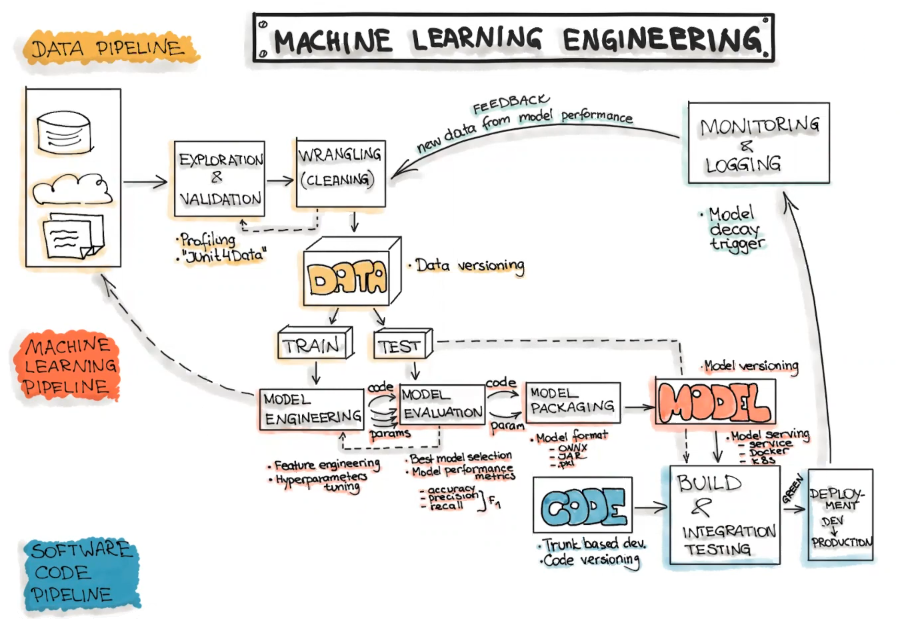
\includegraphics[scale=0.55]{architecture.png}
    \caption{Arquitectura MLOps}
    \label{fig:architecure-mlops}
\end{figure}

\subsubsection{Principios de MLOps}
A continuación, vamos a detallar los principios de MLOps que vamos a seguir en el desarrollo de nuestro proyecto.
En esta sección se incluyen los puntos más importantes de la metodología, durante todo el desarrollo intentaremos
cumplir con ellos en la medida de lo posible, ya que pueden darse situaciones en las que sea totalmente imposible
satisfacerlos al completo.

\begin{itemize}
    \item \textbf{Automatización}: la automatización es la clave para la eficiencia y la escalabilidad.
          Aqui incluimos tareas como la generación de datos, el despliegue del modelo, la evaluación y
          la puesta en producción.
    \item \textbf{Testeo}: garantiza que tanto la funcionalidad como el desempeño del modelo están evaluados correctamente.
          Esencial en Machine Learning para identificar problemas y mejorar la confianza en los resultados.
    \item \textbf{Versionado}: es importante tener un control de versiones de los datos, el código y los modelos.
          Puede variar el método dependiendo de la herramienta que se utilice, pero existen estándares como Git para la gestión
          de código y GitHub/GitLab para el almacenamiento de los repositorios.
    \item \textbf{Reproducibilidad}: es necesario poder reproducir los resultados de forma consistente, puede ser
          complicado en Machine Learning debido a la naturaleza aleatoria de los algoritmos. Igualmente aquí se trataran
          las herramientas y medidas necesarias para lograrlo.
    \item \textbf{Monitorización}: es importante tener un control de los modelos en proceso de entrenamiento o de producción.
          Por ello, recolectar estadisiticas en tiempo de procesamiento nos ayudará a generar nuevas hipotesis para las proximas interaciones.
\end{itemize}

\subsubsection{Flujo de trabajo}
Una de las características de los proyectos de Machine Learning es que son tecnologías en constante evolución, el
desarrollo no es un proceso sencillo y requiere de un enfoque coordinado por parte de los diferentes
equipos que lo conforman para asegurar su sostenibilidad a largo plazo. Es fundamental poder adapatarse a los cambios
de forma agil, sin que esto suponga un deterioro del nivel de productividad o que ralentice el avance de nuevas
funcionalidades.\medskip

Podemos identificar tres fases principales: diseño, desarrollo del modelo y operaciones. Cada fase tiene un enfoque
específico y requiere una serie de tareas para garantizar el éxito del proyecto. La fase de diseño,
se definen los objetivos y requisitos del proyecto, se identifican los datos necesarios para el entrenamiento y
se establecen los criterios de éxito. La fase de desarrollo del modelo, se preparan los datos, se entrena el modelo
y se evalúa su rendimiento. También se realiza la validación y se toman las decisiones sobre el modelo final a utilizar.
Finalmente, en la fase de operaciones, se integra el modelo en la infraestructura existente, se monitorea su rendimiento
y se extraen conclusiones para futuras iteraciones. Al repartir las responsabilidades en diferentes fases, aislamos los erroes junto con la carga de trabajo y podemos avanzar
sin la preocuapacion de que un bug o un cambio requisitos afecte al resto del equipo.

\begin{figure}[ht]
    \centering
    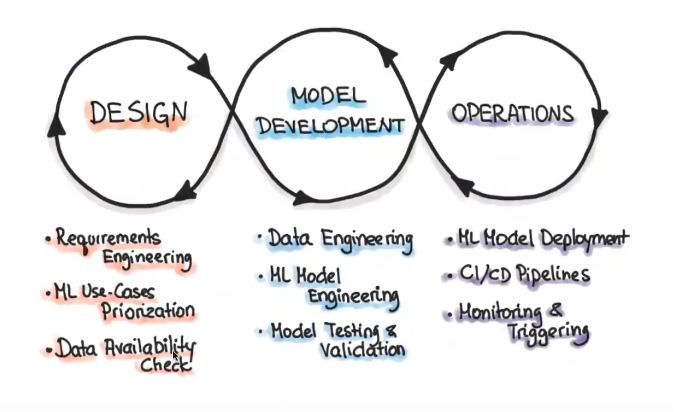
\includegraphics[scale=0.5]{proceso-mlops.png}
    \caption{Metodología MLOps}
    \label{fig:proces-mlops}
\end{figure}

Para visualizar de forma más clara la ventaja que supone este enfoque frente a uno tradicional, a continuación
se mencionara un ejemplos de una posible situacion real. \textbf{Ejemplo:} Tenemos un modelo que actualmente está alojado en AWS y queremos migrarlo a Azure, debido a que
utilizamos MLOps existe configurada una action que en el momento que el equipo publica una nueva release
automáticamente despliega el modelo en el servidor cloud. La parte del equipo encargada de las operaciones procede
a configurar el nuevo servicio y modificar la action para redirigir el despliegue al nuevo servidor. Durante este
tiempo, el equipo de desarrollo a podido avanzar en nuevas mejoras para el modelo y ahora se disponen a volver
a publicar los cambios. Ellos no han notado ningún cambio, pero a nivel de infraestructura se ha realizado una
completa migracion sin afectar en ningún momento en el desarrollo.


\pagebreak
\pagebreak 
    \section{Desarrollo del proyecto}
En esta sección repasaremos los aspectos principales y las especificaciones seguidas 
en el desarrollo de este proyecto. Los principales subtemas que se abordarán son la 
especificación y requisitos del proyecto, el enfoque que se tomó hacia la arquitectura 
y el diseño, una breve inmersión en las tecnologías que se utilizaron, la estrategia de 
pruebas seguida durante el proyecto, consideraciones sobre el entorno de trabajo donde 
se realizó el desarrollo y por último si hubo algún incidente durante el desarrollo.

\subsection{Especificación de Requisitos del Sistema}

\subsubsection{Stakeholders}
Dado que este proyecto es de indole de academica sobre como aplicar 
tecnicas de IL en problemas NP-Hard no tiene clientes directos. Sin embargo, 
teniendo en cuenta hacia qué está enfocado y la utilidad del mismo, se pueden 
identificar 2 tipos de grupos de interes. En primer lugar, los investigadores 
dentro de Tecnalia, ya que un avance en esta problematica les puede servir como punto de partida
para mejorar sus propios algoritmos. En segundo lugar, los clientes de Tecnalia,
ya que podrán utilizar esta herramienta para resolver sus propios problemas de
optimización con unos pequeños ajustes.

\subsubsection{Restricciones Obligatorias}
\begin{itemize}
    \item \textbf{Limitación de tecnologías:} el proyecto esta limitado al uso de
    tecnologías y/o herramientas de código abierto o con licencias apropiadas.
    \item \textbf{Limitación de recursos:} el proyecto esta limitado 
    por recursos como el tiempo, el presupuesto, la disponibilidad de personal, 
    el equipo de hardware y software.
    \item \textbf{Requisitos legales y éticos:} el proyecto esta limitado 
    por los requisitos legales y éticos que deben cumplirse, por ejemplo, en lo 
    que respecta a la privacidad de los datos, la seguridad, la propiedad intelectual 
    y la ética en la investigación.
    \item \textbf{Limitación de acceso a datos:} el proyecto esta limitado
    por el acceso a los datos de los clientes de Tecnalia. En este caso, se
    utilizarán datos generados sinteticamente para poder realizar el proyecto.
\end{itemize}

\subsubsection{Reglas de Negocio}
\begin{itemize}
    \item Al aplicar la metodologia se deben incluir reglas 
    de validación para garantizar que los datos de entrada sean coherentes 
    y estén dentro de los límites aceptables para el problema a resolver.
    \item Se deben establecer los parámetros y procedimientos para el proceso 
    de entrenamiento del modelo de aprendizaje automático que se utilizará 
    para la resolución del problema, incluyendo los criterios de evaluación del modelo.
    \item Se deben especificar las reglas para la interpretación de los resultados 
    obtenidos por la metodología, así como las medidas de calidad que se utilizarán 
    para evaluar el rendimiento de la solución propuesta.
    \item La metodología debe incluir reglas para la gestión de errores
    de la metodología, incluyendo la revisión periódica de las reglas de negocio 
    y la actualización de los modelos de aprendizaje automático.
\end{itemize}
\subsubsection{Catálogo de Requisitos Funcionales}
\begin{enumerate}
    \renewcommand{\labelenumi}{RF\arabic{enumi}}
    \item Se debe proporcionar una definicion clara de los objetivos de la investigación 
    y cómo se van a alcanzar.
    \item Aplicando la metodología debe ser capaz de generar el conjunto de datos de entrenamiento
    y validacion a partir de sistemas de generación de instancias aleatorias.
    \item La metodología debe idenficar diferentes formas para encontrar un experto
    que pueda generar soliciones optimas del caso de uso del problema.
    \item La metodología debe incluir el diseño y entrenamiento de un modelo de Machine Learning 
    adecuado para la tarea específica, de manera que se optimice su precisión y eficiencia.
    \item Aplicando la metodología debe ser capaz de medir y evaluar el rendimiento del modelo 
    utilizando una o varias metricas de calidad específicas para el caso en concreto.
    \item La metodología debe proporcionar un marco para el diseño de la investigación, 
    incluyendo la definición de variables, la identificación de las fuentes de datos y 
    la elección de los métodos de recolección de datos.
    \item La metodología debe incluir la interpretación de los resultados del modelo 
    de Machine Learning, de manera que se puedan extraer conclusiones útiles y relevantes.
\end{enumerate}

\subsubsection{Requisitos no Funcionales}
\begin{enumerate}
    \renewcommand{\labelenumi}{RNF\arabic{enumi}}
    \item La metodología debe ser fácil de entender y utilizar tanto para 
    investigadores expertos como para aquellos que no tienen experiencia en el campo.
    \item La metodología debe ser reproducible por otros investigadores, de manera 
    que los resultados obtenidos puedan ser comparados y validados.
    \item La metodología debe ser lo suficientemente flexible para adaptarse a 
    diferentes situaciones y contextos de investigación.
    \item La metodología debe ser clara y precisa en su presentación y explicación, 
    para evitar ambigüedades y malinterpretaciones.
    \item La metodología debe ser innovadora y estar actualizada con los últimos 
    avances en investigación y tecnología. 
    \item Al desrrolar la metodología se deben seguir los principios de código limpio, 
    utiliar una arquitectura adecuadas y patrones de diseños cuando sea necesario.
\end{enumerate}
\subsection{Especificación del Diseño}
\subsubsection{Arquitectura y entorno tecologico del proyecto}
\paragraph{Arquitectura del software}
La arquitectura del software del modelo está compuesta por cuatro capas principales: 
la capa del modelo, la capa del estado compuesto por un grafo, la capa del 
environment y la capa de ejecución. Se puede ver un diagrama de la arquitectura en la
figura \ref{fig:layers}. \medskip

\begin{itemize}
    \item \textbf{Capa de ejecución:} Esta capa se encarga de ejecutar todo el ecosistema
    del modelo. En nuestro caso es ejecutada por Python 3.10.6 y ofrece la versatilidad de
    poder ejecutar el modelo ya sea en un entorno local o en la nube. 
    \item \textbf{Capa del environment:} Esta capa se encarga de generar el entorno en el que se
    ejecutará el modelo. Cuando se va a resolver un problema de scheduling, el entorno
    prepara todo lo necesario para que el modelo pueda interactuar con el problema y le
    proporciona toda la información necesaria para que pueda tomar decisiones.
    \item \textbf{Capa del estado:} Esta capa se encarga de representar el estado del problema
    mediante un grafo. El grafo representa todas las operaciones que se deben ejecutar y
    las restricciones que existen entre ellas.
    \item \textbf{Capa del modelo:} Esta capa se encarga de resolver el problema de scheduling
    mediante un modelo de Deep Learning. El modelo recibe como entrada el grafo del
    estado y genera como salida una asignación de las operaciones a los recursos. 
\end{itemize}

\begin{figure}[ht]
    \centering
    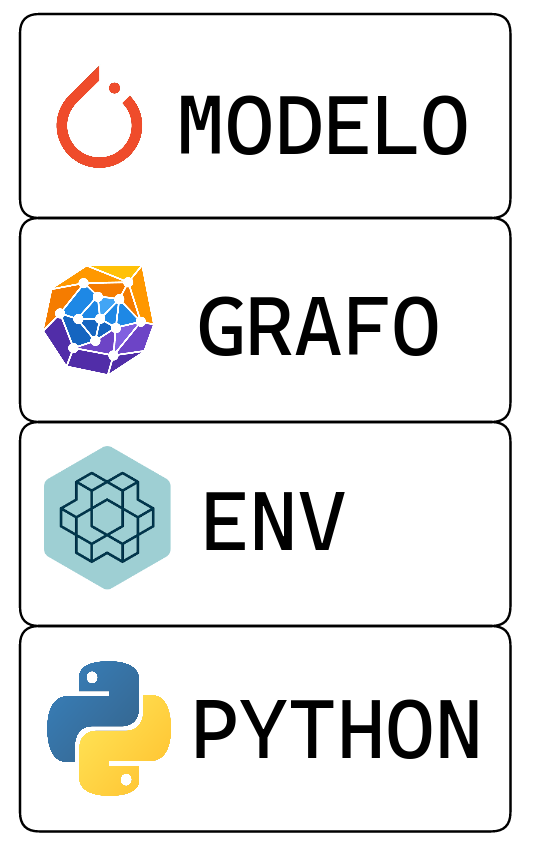
\includegraphics[scale=0.27]{layers.png}
    \caption{Capas de la arquitectura}
    \label{fig:layers}
\end{figure}


\paragraph{Despliegue fisico}
La visualización de los resultados es una parte crítica e importante del proceso. Permite 
a los usuarios finales entender y analizar los datos de una manera más efectiva.  
Sin embargo, es importante destacar que esta parte del proyecto es 
estrictamente opcional y dependerá de las necesidades concretas del caso de uso. 
Si bien la visualización del problema puede ser extremadamente útil algunos casos, puede que no sea 
relevante o necesaria en otros. Por lo tanto, se debe evaluar cuidadosamente la necesidad de 
esta visualización antes de implementarla, ya que puede ser un proceso costoso y 
requerir mucho tiempo.\medskip

\begin{figure}[ht]
    \centering
    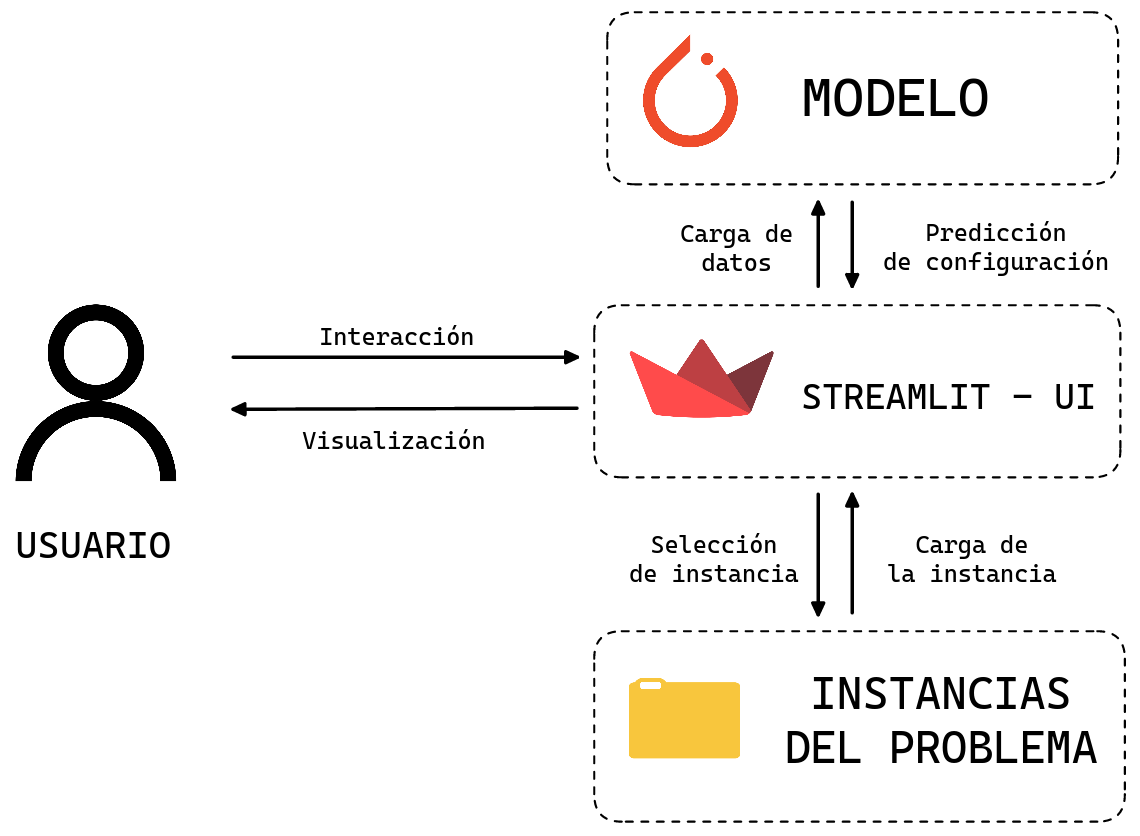
\includegraphics[scale=0.25]{deploy.png}
    \caption{Arquitectura fisica}
    \label{fig:despliegue}
\end{figure}

En este proyecto en particular, se ha optado por se crear una aplicacion web en Streamit 
desde la cual mediante una llamada al modelo generar un gráfico Gantt en el que se podra
visualizar todas las operaciones y sus respectivas asigncaciones y tiempos de ejecucion.
En la figura \ref{fig:despliegue} se puede ver un diagrama del despliegue fisico del modelo.
La aplicacion sirve como intermediario entre el usuario y el modelo, para ello extrae las
diferentes configuraciones de problemas desde una carpeta en la que se encuentran los 
archivos. Lo importante de esta distribucion es que permite una gran versatilidad a la hora
de ejecutar el modelo, ya que se podría mover la ejecución del modelo a un microservicio
externo que se encargue de ejecutar el modelo y devolver los resultados a la aplicacion web.
Para ver más información sobre la aplicación web, se puede consultar el apartado de manual
de usuario donde se explica con más detalle. 

\subsubsection{Descripcion del diseño}
Uno de los diseños más comunmente utilizados para resolver problemas de machine learning
es el uso de sistemas de pipelines. Estos sistemas escapan del paradigma tradicional de
programación secuencial y se basan en la idea de que el problema se puede resolver
mediante la composición de una serie de pasos o etapas. Cada etapa se encarga de realizar
una tarea específica y se comunica con las demás mediante un sistema de colas. De esta
manera, se puede lograr un sistema altamente escalable y flexible. Además, se puede
reutilizar cada etapa para diferentes pipelines o enlazar diferentes pipelines para
conseguir uno más complejo. Otra de las ventajas de este diseño es que permite
abstraer la implementación de cada etapa, lo que permite que cada una de ellas se pueda
mejorar o cambiar sin afectar al resto de ellas, siempre y cuando se mantenga la
interfaz de comunicación.

\subsubsection{Modelo de diseño}
\begin{figure}[ht]
    \centering
    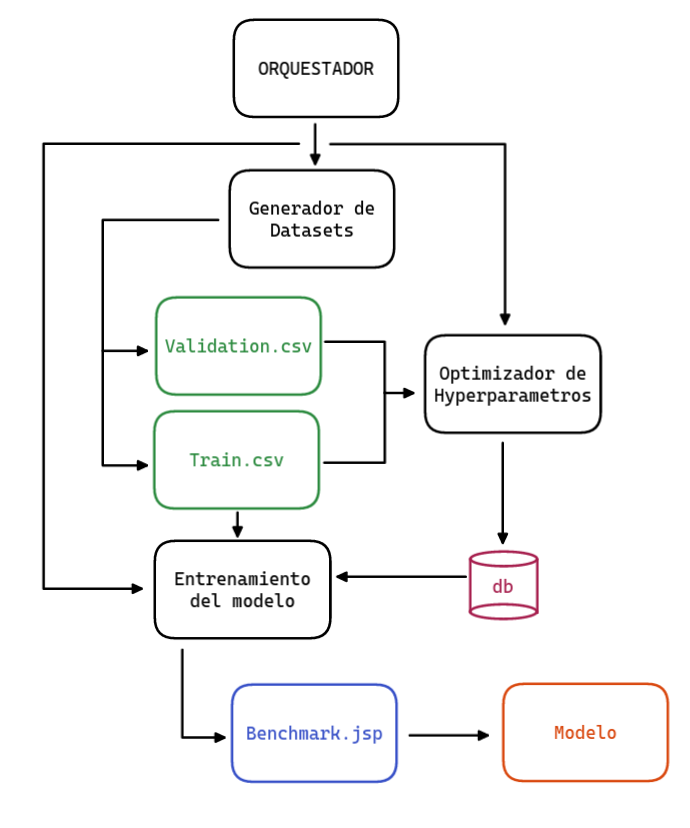
\includegraphics[scale=0.35]{disenio.png}
    \caption{Diseño del sistema}
    \label{fig:desing}
\end{figure}

En la figura \ref{fig:desing} se puede ver al completo las diferentes etapas que componen
el sistema. 

\subsection{Tecnologías Utilizadas}
En la sección se presentarán todas las tecnologías que han tenido un impacto directo en el desarrollo de las 
funcionalidades del proyecto de Machine Learning.

\subsubsection{Python}
Python \cite{C8d} es un lenguaje de programación interpretado de alto nivel. Es una de las herramientas más populares 
en la comunidad de Data Science y Machine Learning debido a su facilidad de uso, su amplia gama de bibliotecas 
y su enfoque en la legibilidad del código. Además, recientemente se está haciendo una tarea de mejora del 
lenguaje con la inclusión de nuevas librerías basadas en C para un mejor rendimiento, inclusión de elementos 
de tipado estático para el mantenimiento del código y mejoras en el sistema de errores.

\subsubsection{NumPy}
NumPy \cite{Numpy} es una biblioteca de Python utilizada para trabajar con matrices y arrays multidimensionales de manera 
eficiente. Fue desarrollada en C++ para ser utilizada en aplicaciones de Data Science y matemáticas, ofrece 
una amplia variedad de funciones y herramientas para operar con matrices y realizar cálculos numéricos complejos. 
Además, al estar escrito en C++ está altamente optimizado para trabajar con grandes conjuntos de datos, realizar 
operaciones aritméticas y lógicas, de indexar y redimensionar matrices de manera eficiente, realizar transformaciones 
de Fourier y realizar cálculos de álgebra lineal.

\subsubsection{Pandas}
Pandas \cite{pandas} es una biblioteca de Python utilizada para la manipulación y análisis de datos. Es especialmente 
útil para el manejo de grandes conjuntos de datos y ofrece una variedad de herramientas y funciones para 
trabajar con diferentes tipos de datos y formatos. Una de las estructuras de datos principales de Pandas es 
el DataFrame, que se puede considerar como una tabla de datos bidimensional, donde cada fila representa una 
observación y cada columna representa una variable. Los DataFrames permiten la manipulación y transformación 
de datos mediante una variedad de operaciones, lo que los hace muy útiles en aplicaciones de ciencia de datos 
y análisis de datos. 

\subsubsection{PyTorch}
PyTorch \cite{PyTorch} es un framework de código abierto de Deep Learning hecho en Python, desarrollado por el equipo 
de Inteligencia Artificial de Facebook. Se utiliza para crear y entrenar modelos de redes neuronales para resolver 
problemas de Machine learning. PyTorch es muy popular en la comunidad de investigación debido a su facilidad de uso 
y su capacidad para realizar cálculos en GPU para acelerar el proceso de entrenamiento de modelos. Además, PyTorch
ofrece una gran variedad de herramientas y funciones para trabajar con redes neuronales, como la creación de
diferentes tipos de redes neuronales, la definición de funciones de pérdida, la definición de optimizadores, la 
definición de funciones de activación, etc.

\subsubsection{Gym}
Gym \cite{Gym} es una biblioteca de Python utilizada para el diseño y creación de environments de RL. Incluye un 
gran conjunto de herramientas para trabajar con algoritmos personalizados y ofrece muchas facilidades en 
el registro y monitorización del proceso de entrenamiento. Todas estas razones lo convierte en la opción más popular 
para los desarrolladores cuando abordan problemas de RL.

\subsubsection{PyTorch Geometric}
PyTorch Geometric \cite{pytorch-geometric} es una librería que ofrece soporte para el procesamiento de grafos, lo que significa 
que se puede utilizar para trabajar con redes de datos en las que los nodos están conectados por enlaces. 
Esto puede ser útil ya que mediante técnicas de Deep Learning se puede analiza la estructura y las 
relaciones que existen entre los nodos de un grafo y extraer de ahi sus características. Además, la 
librería ofrece herramientas para trabajar con diferentes tipos de grafos, como grafos dirigidos y heterogéneos, 
que son los utilizados en el proyecto, y proporciona una serie de funciones para realizar 
operaciones básicas con grafos.

\subsubsection{Or-tools}
OR-Tools \cite{ortools} es una biblioteca de optimización combinatoria de código abierto para Python y otros 
lenguajes de programación. Permite resolver problemas de optimización de manera eficiente, utilizando una 
amplia variedad de algoritmos y técnicas de programación matemática. Con OR-Tools, los usuarios pueden 
resolver problemas de programación lineal, programación entera mixta, programación cuadrática, 
problemas de rutas y muchos otros. Además, la biblioteca también incluye herramientas para resolver 
problemas de programación con restricciones, como la asignación de tareas o la programación de horarios.

\subsubsection{Optuna}
Optuna \cite{optuna_2019} es una biblioteca de optimización de hiperparámetros de código abierto para Python. Su objetivo 
es automatizar el proceso de ajuste de hiperparámetros, que a menudo es un proceso intensivo en 
recursos y muy demandante en tiempo, para permitir a los usuarios encontrar la mejor configuración 
de hiperparámetros de sus modelos de Machine Learning de manera eficiente. Optuna utiliza algoritmos 
de optimización Bayesiana \cite{Ye_2020} para buscar los mejores valores de hiperparámetros en función del 
rendimiento de los modelos en el conjunto de validación. Con Optuna, los usuarios pueden definir una función 
objetivo y especificar los rangos de búsqueda de cada hiperparámetro, así como las restricciones entre ellos, 
lo que permite a la biblioteca ajustar varios hiperparámetros al mismo tiempo.

\subsubsection{Streamlit}
Streamlit \cite{Streamlit} es una biblioteca de Python que permite a los usuarios crear aplicaciones web interactivas
para Machine Learning y Data Science. Proporciona una serie de herramientas y widgets preconstruidos 
que permiten a los desarrolladores agregar fácilmente gráficos, tablas, mapas y otros tipos de 
visualizaciones a sus aplicaciones. Además, se integra bien con bibliotecas populares de Python 
para el procesamiento de datos y el aprendizaje automático, como Pandas, NumPy y Scikit-Learn \cite{scikit-learn}.
Streamlit se ejecuta en un servidor local y los usuarios interactúan con la aplicación a través 
de un navegador web. Esto hace que sea fácil compartir aplicaciones y colaborar en ellas.
\subsection{Consideraciones sobre la Implementación}
\subsubsection{Estructura del codigo}
La estructura del codigo se ha diseñado para que sea lo más modular posible,
de forma que cada modulo tenga una única responsabilidad y sea fácilmente
intercambiable. La distribucion de ficheros y carpetas se puede ver en la 
\textbf{Figura \ref{fig:estrcutra-ficheros}}.

\begin{figure}[ht]
\dirtree{%
    .1 /.
    .2 Makefile.
    .2 README.md.
    .2 pyproject.toml.
    .2 .pre-commit-config.yaml.
    .2 requirements.txt.
    .2 src.
    .3 \_\_init\_\_.py.
    .3 app.py.
    .3 main.py.
    .3 config.
    .4 hyperparams.py.
    .4 settings.py.
    .3 environment.
    .4 fjspenv.py.
    .4 generator.py.
    .4 graph.py.
    .4 solver.py.
    .3 model.
    .4 actor.py.
    .4 eval\_model.py.
    .4 train\_model.py.
    .3 pipes.
    .4 generate\_data.py.
    .4 generate\_optimun.py.
    .4 generate\_training.py.
    .4 generate\_validation.py.
    .3 utils.
    .4 parsedata.py.
    .2 test.
    .3 fjspenv\_test.py.
    .3 graph\_test.py.
    .3 pipeline\_test.py.
}
\caption{Estructura de ficheros del proyecto}
\label{fig:estrcutra-ficheros}
\end{figure}

A continuación se detallan las carpetas y ficheros más importantes del proyecto:
\begin{itemize}
    \item \textbf{src: } Contiene todo el código ejecutable del proyecto, siendo \textit{main.py} el archivo 
    principal que se ejecuta para lanzar el proyecto. Este archivo se encarga de cargar los
    diferentes módulos y realizar las llamadas a las pipelines para generar los datos de entrenamiento,
    validación, así como ejecutar el entrenamiento y la evaluación del modelo. También existe un archivo
    \textit{app.py} que se encarga de cargar la demo del proyecto mediante una pagina web y ejecutar el 
    algoritmo de resolución.
    \item \textbf{config: } Contiene el archivo de configuración de los hiperparámetros para el entrenamiento 
    y las diferentes variables de configuración del proyecto.
    \item \textbf{environment: } Contiene los archivos relacionados con el environment del problema, como la
    clase que representa el grafo heterogeneo, el environment de OpenAI Gym, el generador de instancias y 
    el resolutor de las mismas.
    \item \textbf{model: } Contiene los archivos relacionados con el modelo de aprendizaje profundo, como la
    clase que representa la red neuronal, el entrenador y el evaluador del modelo.
    \item \textbf{pipes: } Contiene los archivos relacionados con las pipelines de generación de datos,
    validación y entrenamiento. 
    \item \textbf{utils: } Contiene los archivos de utilidades, como el parser de los datos de entrada.
    \item \textbf{test: } Contiene los archivos de testeo de los módulos.
\end{itemize}

\subsubsection{Entorno de desarrollo}
El desarrollo del proyecto se ha realizado en un entorno Linux, concretamente en un sistema operativo
Arch Linux. El editor de código utilizado ha sido Visual Studio Code, que es un editor de código
de código abierto desarrollado por Microsoft. Este editor de código es uno de los más utilizados
en la actualidad y cuenta con una gran comunidad de desarrolladores que desarrollan extensiones
para el mismo. En este proyecto se ha utilizado la extensión de Python para Visual Studio Code,
que permite ejecutar código Python directamente desde el editor de código, así como depurar el
código y ejecutar tests. También se ha utilizado otras extensiones como GitHub Copilot, que es
una extensión que utiliza inteligencia artificial para sugerir código al desarrollador y amVim
que es una extensión que permite utilizar el editor de código como si fuera el editor Vim.

\subsubsection{Gestión de dependencias y reproducibilidad}
La gestión de dependencias y la reproducibilidad es uno de los temas de mayor importancia en el 
desarrollo de un proyecto de software. En el caso de este proyecto, se ha optado por utilizar 
un kit de herramientas para garantizar que el proyecto se pueda ejecutar siempre en las mismas 
condiciones. Para ello, se va ha fijar la versión de Python a la 3.10.6 y el resto de dependencias. 

\begin{itemize}
    \item \textbf{Pyenv: } Pyenv es un administrador 
    de versiones de Python que permite tener múltiples versiones de Python instaladas en un mismo sistema 
    y cambiar fácilmente entre ellas. Con Pyenv, es posible instalar distintas versiones de 
    Python y asegurarse de que el código se está ejecutando en la versión correcta. 
    
    \item \textbf{Virtualenv: } Virtualenv es una herramienta que permite crear entornos virtuales de Python para trabajar 
    en proyectos específicos. Cada entorno virtual puede tener su propia versión de Python y bibliotecas instaladas, 
    lo que permite aislar proyectos y evitar conflictos entre versiones y dependencias. Con Virtualenv, 
    es posible instalar y gestionar paquetes de Python específicos para cada proyecto, sin afectar 
    al sistema operativo global.

    \item \textbf{Pip-Tools: } Pip-Tools es una herramienta de línea de comandos para la gestión de 
    dependencias de Python. Permite especificar las dependencias de un proyecto en un archivo 
    "pyproject.toml" y asegurarse de que se instalen y se mantengan actualizadas todas las dependencias 
    de manera controlada. También permite generar archivos "requirements.txt" en el que se especifican las 
    versiones exactas de todas las dependencias, lo que ayuda a garantizar que la reproducibilidad del 
    proyecto se mantenga consistentes y se instalen correctamente.

\end{itemize}


\subsubsection{Gestión de la calidad del codigo}
Al igual que la gestión de dependencias, la gestión de la calidad del código es un tema de gran importancia
ya que permite mantener un código limpio, legible y fácil de mantener. Para ello, se ha optado por utilizar
una serie de medidas y herramientas que permiten mantener la calidad del código a lo largo del desarrollo del proyecto.
Entre estas medidas se incluyen liteners de código, formateadores de código, analizadores estáticos de código y
herramientas de pruebas unitarias. A continuación se detallan la lista de herramientas:

\begin{itemize}
    \item \textbf{Git: } Git es un sistema de control de versiones distribuido que se utiliza para el 
    seguimiento y gestión del código fuente. Permite a los desarrolladores trabajar en el mismo código fuente 
    sin necesidad de coordinar su trabajo constantemente. Ofrece la posibilidad de volver a versiones anteriores en 
    caso de errores o cambios no deseados, paralelismo de trabajo mediante el uso de diferentes ramas y cuenta 
    con multitud de plataformas web como Github o Gitlab para el almacenamiento de repositorios en remoto.

    \item \textbf{Pre-commit: } Pre-Commit es una herramienta que se utiliza para garantizar que el código 
    fuente de un proyecto cumpla con un conjunto de reglas y estándares de calidad antes de que se realice 
    un commit. Pre-Commit se integra con Git y se ejecuta automáticamente antes de cada commit, lo que ayuda 
    a garantizar que el código se mantenga limpio y organizado. Se configura mediante un archivo llamado 
    ".pre-commit-config.yaml", que especifica las herramientas que se utilizarán para verificar el código 
    y viene con una gran cantidad de herramientas integradas, incluyendo linters de Python, comprobadores 
    de estilo de código, herramientas de seguridad, etc. También es posible agregar herramientas 
    personalizadas si es necesario.

    \item \textbf{Ruff:} Ruff es un linter de Python escrito en Rust, es decir una herramienta de 
    análisis estático de código que ayuda a identificar errores de sintaxis, errores de estilo y posibles 
    problemas de rendimiento en el código fuente de un programa. Además, el hecho de que RUFF esté escrito 
    en Rust le da una ventaja en cuanto a velocidad y eficiencia, el uso de Rust significa que RUFF se 
    ejecutará rápidamente y consumirá pocos recursos del sistema, lo que puede ser especialmente beneficioso 
    para proyectos de gran tamaño.

    \item \textbf{Black: } Black es un formateador de código para Python que se utiliza para garantizar
    que el código cumpla con las directrices de estilo de Python PEP 8, lo que mejora la legibilidad 
    del código y ahorra tiempo de desarrollo. Se integra fácilmente en flujos de trabajo existentes 
    y es altamente configurable para adaptarse a diferentes estilos de formato. Black es compatible 
    con diferentes versiones de Python y es una herramienta valiosa para cualquier equipo de desarrollo 
    de Python que busque mejorar la calidad y consistencia del código.

    \item \textbf{Mypy: } Mypy es una herramienta de análisis estático para Python que permite a los 
    desarrolladores verificar el tipado estático de su código. Al analizar el código para detectar 
    problemas de tipado, Mypy ayuda a prevenir errores comunes, mejorar la comprensión del código 
    y ofrece una mayor capacidad de mantenimiento a largo plazo.
    
\end{itemize}


\subsection{Plan de Pruebas}
Como parte del proceso de desarrollo del proyecto, se ha llevado a cabo un riguroso 
proceso de testeo para asegurar el correcto funcionamiento del mismo. Es importante 
destacar que, debido a la naturaleza de un proyecto de investigación, sólo se han 
testado las funcionalidades fundamentales del proyecto, es decir, aquellas que 
son críticas para el cumplimiento de los objetivos de la investigación. Es poco 
probable que estas funcionalidades sufran cambios significativos, por lo que se ha 
prestado especial atención en asegurar que estén libres de errores y funcionen correctamente.\medskip

Se ha utilizado Pytest que es un framework de testing de software para escribir, 
organizar y ejecutar pruebas unitarias automatizadas. Es una herramienta popular 
debido a su sintaxis sencilla y fácil de aprender, además de su capacidad para detectar 
reportar errores de manera clara y concisa. Pytest permite a los desarrolladores 
escribir pruebas más legibles, organizadas y mantenibles con menos código 
que otras alternativas. 

\begin{figure}[ht]
    \label{fig:pytest-output}
    \begin{lstlisting}
=========================== test session starts ===================
platform linux -- Python 3.10.6, pytest-7.3.0, pluggy-1.0.0
rootdir: /home/betagmr/dev/fjsp
configfile: pyproject.toml
collected 15 items                                                         

test/graph_test.py ...........                               [ 58%]
test/environment/fjspenv_test.py ......                      [ 89%]
test/model/eval_model_test.py .                              [ 94%]
test/virtualenv/version_test.py .                            [100%]

============================ 19 passed in 1.77s =================== 
    \end{lstlisting}
    \caption{Ejecución de las pruebas unitarias con Pytest}
\end{figure}

En la figura \ref{fig:pytest-output} se puede ver la salida de la ejecución de las
pruebas unitarias. En este caso, se han ejecutado 19 pruebas unitarias, de las cuales
ofrecen un 60\% de cobertura del código total y un 100\% de cobertura de las funcionalidades
fundamentales del proyecto. Se considerean funcionalidades fundamentales aquellas que
están relacionadas con la gestión de los grafos, el environment y la evaluación de los
modelos.

\subsection{Incidencias del Proyecto}
En esta sección del TFG, se aborda uno de los aspectos más importantes del desarrollo 
de un proyecto de Machine Learning: los problemas y desafíos que pueden surgir durante 
el proceso. Es común que se presenten dificultades que pueden afectar tanto la precisión 
como la eficiencia del modelo. Estos problemas pueden ser causados por una variedad 
de factores a continuación se describen algunos de los inconvenientes que se presentaron
durante el desarrollo del proyecto.

\subsubsection{Problemas con la normalización de los datos}
La normalización de los datos de entrada es un paso crítico para garantizar que el 
modelo pueda aprender de manera efectiva y generar predicciones precisas. En el caso 
específico de los grafos, el estado de un nodo puede almacenar diferentes tipos de datos, 
como números, referencias a otros nodos, etc, lo que puede generar problemas a la hora 
de la normalización. Otro lugar done también surgen problemas de normalización es en los 
datos de las aristas, que representan las conexiones entre nodos. Al respresentar un 
nodo como una lista de características, estas diferentes caracteristicas de pueden 
requerir de diferentes técnicas de normalización.\medskip

La soluación que se ha adoptado en este proyecto es la de normalizar los datos de
cada entrada de manera independiente. De esta manera, se evitan problemas de colision 
entre los diferentes nodos y aristas de un mismo grafo. Esta solución, sin embargo,
trae problemas de escalabilidad ya que cada vez que se implementa y/o añade una nueva
característica al modelo, es necesario modificar el código de normalización de los datos.\medskip

En un futuro, se podría implementar una solución más escalable, que permita definir
un conjunto de tipos de características con sus respectivas técnicas de normalización.
De este modo, se podría añadir nuevas características al modelo sin necesidad de
modificar el código de normalización. Además, también daría la posibilidad de
poder en una fase de test, probar diferentes técnicas de normalización para
cada tipo de característica y elegir la que mejor se adapte al modelo.

\subsubsection{Problemas con el hardware de entrenamiento}
La falta de hardware adecuado para el entrenamiento y test es un problema común 
que puede afectar la eficiencia y la precisión del modelo. El entrenamiento de modelos 
de Machine Learning a menudo requiere una gran cantidad de recursos computacionales, 
como procesadores, memoria RAM y capacidad de almacenamiento. Además, los modelos 
pueden requerir GPUs (unidades de procesamiento gráfico) especializadas para acelerar 
el proceso de entrenamiento.\medskip

La falta de hardware adecuado puede limitar la cantidad de datos que se pueden usar 
para entrenar el modelo, la complejidad del modelo que se puede entrenar y la 
velocidad a la que se puede realizar el entrenamiento. Esto puede resultar en 
modelos que no sean lo suficientemente precisos o que no se puedan entrenar en 
un tiempo razonable. En el caso de este proyecto, se ha contado con un pequeño
servidor que disponía de una CPU y 4GB de RAM, lo que ha limitado el tamaño de los
grafos que se han podido usar para el entrenamiento. Además, el entrenamiento de
los modelos y la búsqueda de hiperparámetros ha sido un proceso lento, ya que
no se ha contado con una GPU para acelerar el proceso.\medskip

En un futuro, se podría implementar una solución que permita entrenar los modelos
utilizando una o varias GPUs. Esto permitiría entrenar modelos más complejos
con un mayor número de parámetros y con un mayor número de datos de entrenamiento.

\subsubsection{Problemas de rendimiento}
Python es un lenguaje de programación interpretado, lo que significa que el código
se ejecuta línea por línea, en lugar de compilarlo en un programa ejecutable. Esto
hace que sea extremadamente lento en comparación con otros lenguajes de programación
como es el caso de C o C++. Es por ello que durante el desarrollo del proyecto, se
ha tenido que realizar varias tareas de profiling para identificar las partes del
código que más tiempo de ejecución consumían y optimizarlas.\medskip

Para ello se ha utilizado la librería \textit{cProfile} de Python, que permite
realizar un análisis de rendimiento del código. Esta librería genera un informe
con el número de llamadas y el tiempo de ejecución de cada función del código.
De este modo, se puede identificar las funciones que más tiempo de ejecución
consumen y optimizarlas.\medskip

\begin{figure}
    \centering
    \begin{minipage}{0.47\textwidth}
        \centering
        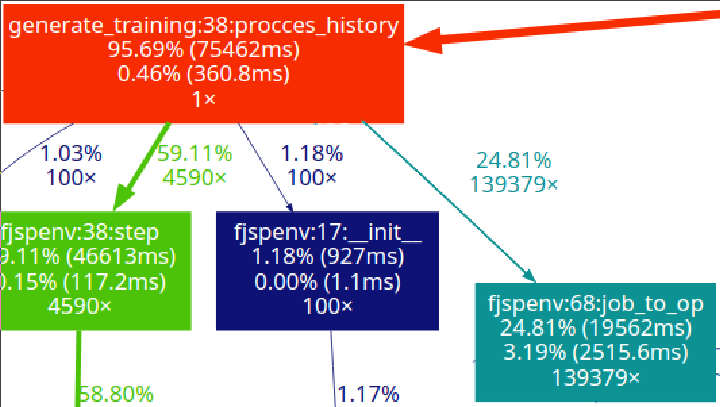
\includegraphics[width=0.85\textwidth]{before-fix.png} 
        \caption{Environment no optimizado}
    \end{minipage}\hfill
    \begin{minipage}{0.47\textwidth}
        \centering
        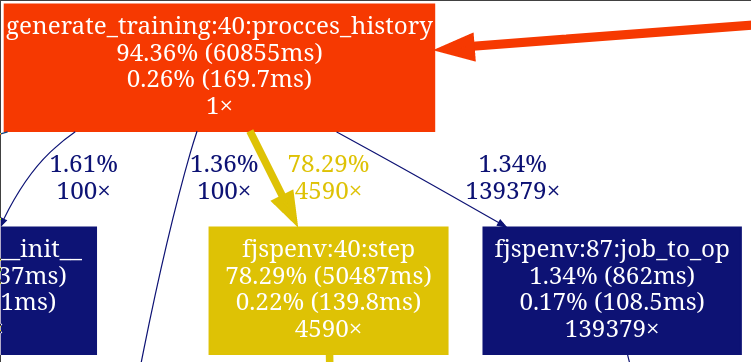
\includegraphics[width=1\textwidth]{after-fix.png}
        \caption{Environment optimizado}
        \label{fig:after-fix}
    \end{minipage}
\end{figure}

En este caso en concreto en el que se puede ver la diferencia de rendimiento
entre el código no optimizado y el código optimizado, debido a que la función
\textit{job\_to\_op} del environments que se encarga de transformar un trabajo
en una operación para poder actualizar el estado del grafo, se ejecuta un gran
número de veces durante el entrenamiento. Por ello, se ha optimizado el código
de esta función para que sea más eficiente utilizando una utilidad de Python
llamada \textit{functools.lru\_cache}, que permite cachear los resultados de
una función para evitar tener que ejecutarla varias veces con los mismos
parámetros.\medskip

Como se puede ver en la figure \ref{fig:after-fix}, el tiempo de ejecución
se ha reducido un 24\% del tiempo total de ejecución del código. Si quisiéramos
optimizar aún más el código, se podría implementar algunas de las funciones
del environment en C++ y luego importar el módulo en Python, aunque esto
requeriría un mayor esfuerzo de desarrollo. 
\pagebreak
    \section{Proceso del desarrollo del proyecto}
\subsection{Modelado del problema}
El modelado del problema es una de los campos con mayor potencial dentro del FJSP, trabajar sobre una 
propuesta solida puede repercutir directamente en el resultado final, por lo que es necesario
contemplar diferentes alternativas. En este apartado se desarrollará la propuesta final exclusivamente,
pero se hará referencia a otras alternativas que se han descartado dentro de la sección de "Posibles
representaciones del problema".

\subsubsection{Procedimiento para definir un environment de RL}
El RL es un tipo de aprendizaje automático que se basa en la interacción de un agente con el environment. 
Este agente toma decisiones en función de la información que recibe del estado y es recompensado 
o penalizado acorde a las decisiones que toma y su objetivo es maximizar la recompensa total 
obtenida a lo largo del tiempo. Este tipo de técnicas se pueden utilizar para resolver problemas de optimización 
combinatoria en los que el espacio de estados es muy grande y no es posible explorar todas sus combinaciones. 
En casos en los que el espacio de estado del problema es muy grande o cambia continuamente,
el aprendizaje por refuerzo puede ser útil para encontrar soluciones óptimas sin necesidad de
explorar todo el espacio de estado. Podemos definir un environment de RL formalmente de la siguiente manera:

\begin{itemize}
    \item \textbf{Espacio de estados ($\boldsymbol{\mathcal{S}}$):} Es el conjunto de todos los posibles estados del environment. 
    Puede ser finito o infinito, y se denota como $\mathcal{S} = \{s_1, s_2, ..., s_n\}$, donde si $\mathcal{S}$ es finito, $n$ representa 
    el número de estados posibles. Por ejemplo, si estuviéramos modelando un juego de ajedrez, el espacio 
    de estados incluiría todas las posibles configuraciones del tablero.

    \item \textbf{Espacio de acciones ($\boldsymbol{\mathcal{A}}$):} Es el conjunto de todas las posibles acciones que un agente 
    puede tomar en el environment. Al igual que el espacio de estados, el espacio de acciones puede ser finito 
    o infinito, y se denota como $A = \{a_1, a_2, ..., a_m\}$, donde si es finito, $m$ representa el número de 
    acciones posibles. Siguiendo con el ejemplo del juego de ajedrez, el espacio de acciones podría incluir 
    todos los posibles movimientos que un jugador puede hacer en su turno.

    \item \textbf{Función de transición de estados ($\boldsymbol{T}$):} Es una función que define la probabilidad de transición 
    de un estado a otro estado dado una acción tomada por el agente. Se denota como $T(s, a, s')$, donde $s$ es el 
    estado actual, $a$ es la acción tomada y $s'$ es el siguiente estado alcanzado después de tomar la acción a en 
    el estado $s$. Formalmente, la función de transición se puede escribir como: 
    $T: \mathcal{S} \times \mathcal{A} \times \mathcal{S'} \ \rightarrow \ [0,1]$, donde 
    [0, 1] representa el rango de probabilidades.

    \item \textbf{Función de recompensa ($\boldsymbol{R}$):} Es una función que asigna una recompensa numérica a una transición 
    de estado y acción específica. Se denota como $R(s, a, s')$, donde $s$ es el estado actual, a es la acción tomada, 
    $s'$ es el siguiente estado alcanzado después de tomar la acción $a$ en el estado $s$, y $R(s, a, s')$ es 
    la recompensa asociada a esa transición. Formalmente, la función de recompensa se puede escribir 
    como: $R: S x A x S -> R$, donde R es un valor numérico que representa la recompensa. 
\end{itemize}

\textbf{Nota: } En nuestro caso, no será necesario definir una función de recompensa, ya que debido a la 
naturaleza del Imitation Learning no requiere de una función de recompensa. Esto se debe a que el agente 
no toma decisiones por si mismo, sino que aprende a tomar decisiones a partir de un experto.

\subsubsection{Representación del estado}
\paragraph{Grafos heterogéneos}
La propuesta del estado se basa en una representación mediante el uso de un grafo heterogéneo. Un grafo 
heterogéneo es un tipo de grafo en el que los nodos y/o aristas pueden tener diferentes tipos, atributos 
y propiedades. Esto significa que se pueden representar diferentes relaciones, y pueden tener distintas 
características asociadas a ellas. Por ejemplo, en un caso donde se quiera modelar una red social, 
los nodos podrían representar personas, contenidos o grupos y las aristas amistades, seguidores, 
miembros de un grupo, etc.\medskip 

En el caso del FJSP es posible representar las operaciones, máquinas y trabajos como nodos del grafo, 
y a su vez las aristas se pueden utilizan para asignar las restricciones y características del problema, como los tiempos de 
procesamiento, las dependencias entre tareas y la asignación de las mismas. Esto permite una representación 
compacta de la información relevante del problema, siendo una de sus virtudes que, a medida que se aumenta 
el número de máquinas y operaciones, simplemente se agregarán más nodos y aristas al grafo, lo que no 
implicara un aumento exponencial en la complejidad de la representación, permitiendo asi una escalabilidad 
natural en términos de la representación del problema. Otra de sus ventajas es que las operaciones sobre 
grafos, como la búsqueda o manipulación de nodos y aristas, son operaciones computacionalmente eficientes. 
Esto permite realizar cálculos y análisis en tiempo razonable, incluso cuando el tamaño del problema incrementa. 

\begin{figure}[ht]
    \centering
    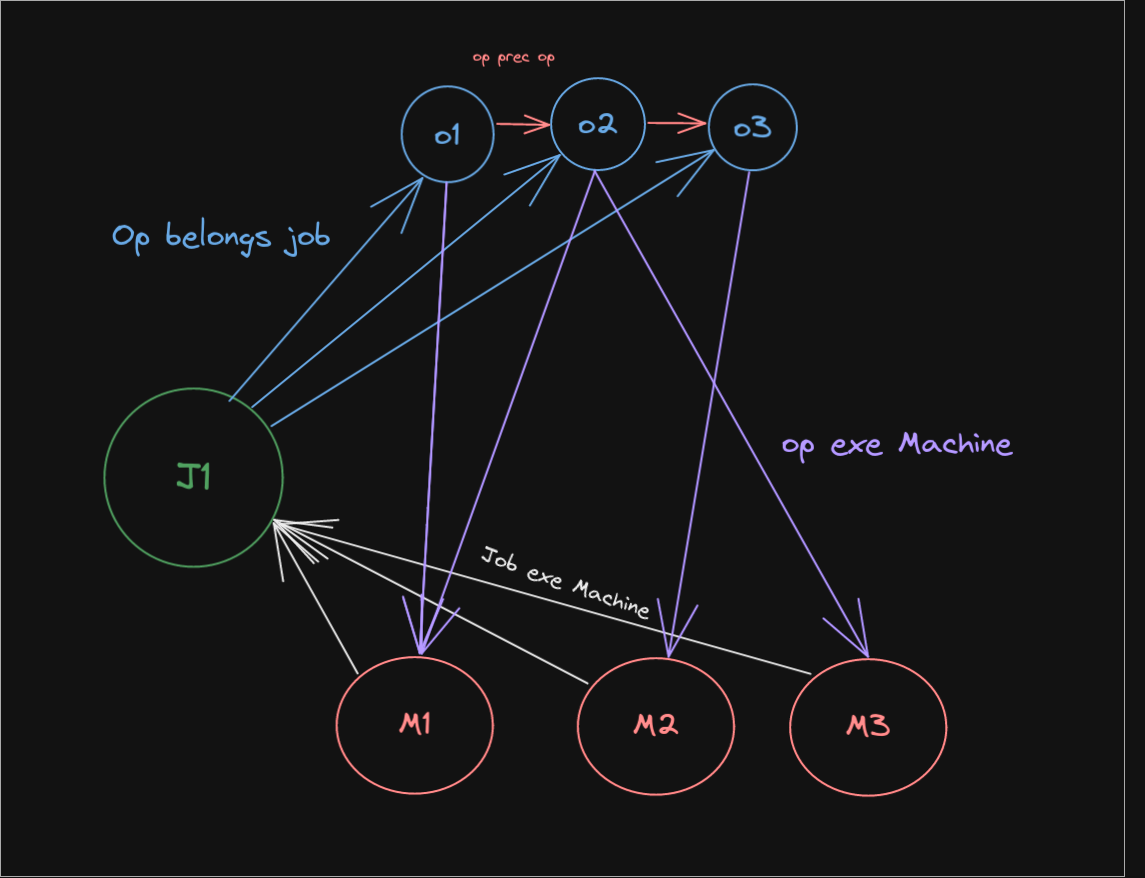
\includegraphics[scale=0.34]{graphv1.png}
    \caption{Ejemplo simplificado de un grafo heterogéneo para el FJSP}
    \label{fig:grafo-heterogeneo}
\end{figure}

Como se puede ver en la Figura \ref{fig:grafo-heterogeneo}, hemos representado mediante un grafo
heterogéneo una instancia del FJSP que cuenta con 3 máquinas, 1 trabajo y 3 operaciones. En este caso, 
la operación 1 solo puede ser ejecutada en la máquina 1 y es por ello que no está conectada con 
las otras máquinas mediante la relación `Operación Ejecuta Máquina'. Aclarar que por motivos de 
simplificación, no se han incluido todos los diferentes tipos de relaciones existentes entre 
los nodos y solo están representadas las relaciones más importantes. Se debe tomar como una ayuda 
visual para entender el potencial que tiene este tipo de representaciones, durante las siguientes 
secciones detallaremos en profundidad todas las características de los nodos y de sus relaciones.

\paragraph{Tipos de nodos y sus características}
\begin{itemize}
    \item \textbf{Operación ($\boldsymbol{\mathcal{O}}$):} La operación es la unidad fundamental de trabajo en el FJSP. Cada 
    operación tiene un identificador único, un flag que indica si ha sido ejecutada,
    un flag que indica si es posible ejecutar la operación y el número de máquinas en las que puede
    ser ejecutada.
    \item \textbf{Trabajo ($\boldsymbol{\mathcal{J}}$):} Representa un conjunto de operaciones que deben ser ejecutadas 
    en una secuencia determinada. Cada trabajo tiene un identificador único, el tiempo de 
    procesamiento de la ultima operación que ha sido procesada, el numero de operaciones restantes y el gap total
    existente entre todas las operaciones del job.
    \item \textbf{Máquina ($\boldsymbol{\mathcal{M}}$):} Representa una máquina dentro del problema del FJSP. Cada máquina 
    cuenta con un identificador único, el tiempo de procesamiento acumulado de todas sus operaciones,
    el gap total existente entre todas las operaciones de la máquina y la diferencia entre el tiempo
    de procesamiento entre ella y la máquina con menor tiempo de procesamiento.  
\end{itemize}

\paragraph{Tipos de relaciones entre nodos}
\begin{itemize}
    \item \textbf{Operación - precede - Operación:} Esta relación indica que la operación 1 debe ser
    ejecutada antes que la operación 2. Se utiliza para representar las dependencias entre operaciones
    dentro de un mismo trabajo.
    \item \textbf{Operación - pertenece - Trabajo:} Esta relación indica que la operación 1 pertenece
    al trabajo 1. Se utiliza para representar las dependencias entre operaciones y trabajos.
    \item \textbf{Trabajo - escucha - Trabajo:} Relación auxiliar que se utiliza para conectar los
    nodos de trabajo y proveer de información a los nodos de la red.
    \item \textbf{Trabajo - escucha - Máquina:} Relación auxiliar que se utiliza para conectar los
    nodos de trabajo con los nodos y máquina para proveer de información a los nodos de la red.
    \item \textbf{Máquina - escucha - Trabajo:} Similar a la relación anterior, pero en este caso
    las relaciones se establecen en sentido opuesto.
    \item \textbf{Operación - ejecuta - Máquina:} Relación entre las operaciones y las máquinas que indica
    que la operación 1 puede ser ejecutada en la máquina 1. Esta relación cuenta con un atributo que
    indica el tiempo de procesamiento de la operación 1 en la máquina 1.
    \item \textbf{Máquina - ejecuta - Trabajo}: Relación directa entre la máquina y el trabajo, esta
    relación indica que la máquina 1 ejecuta el trabajo 1. Adicionalmente, esta relación cuenta con
    un atributo que indica el tiempo de procesamiento de la operación que se está ejecutando en el
    trabajo 1 para la máquina 1.
    \item \textbf{Máquina - gap - Trabajo}: Misma relación que la anterior, pero esta intercambia el
    atributo de tiempo de procesamiento por el gap que generaría la operación que se está ejecutando
    en el trabajo 1 si se llegase a aplicar en la máquina 1.
\end{itemize}

\paragraph{Representación final}
Para finalizar, se muestra la representación que tendría un estado tomando en consideración el ejemplo 
de la Figura \ref{fig:example-solution} utilizada en la introducción. En la siguiente figura ahora ya 
se pueden apreciar todas las relaciones mencionadas con anterioridad, y para conocer en mayor profundidad
como se ha implementado puede consultar la sección de desarrollo. Hemos querido continuar con el ejemplo
que se ha utilizado en la introducción y en el resto de la sección también se hará referencia a este
para ilustrar las futuras explicaciones. 

\begin{figure}[ht]
    \centering
    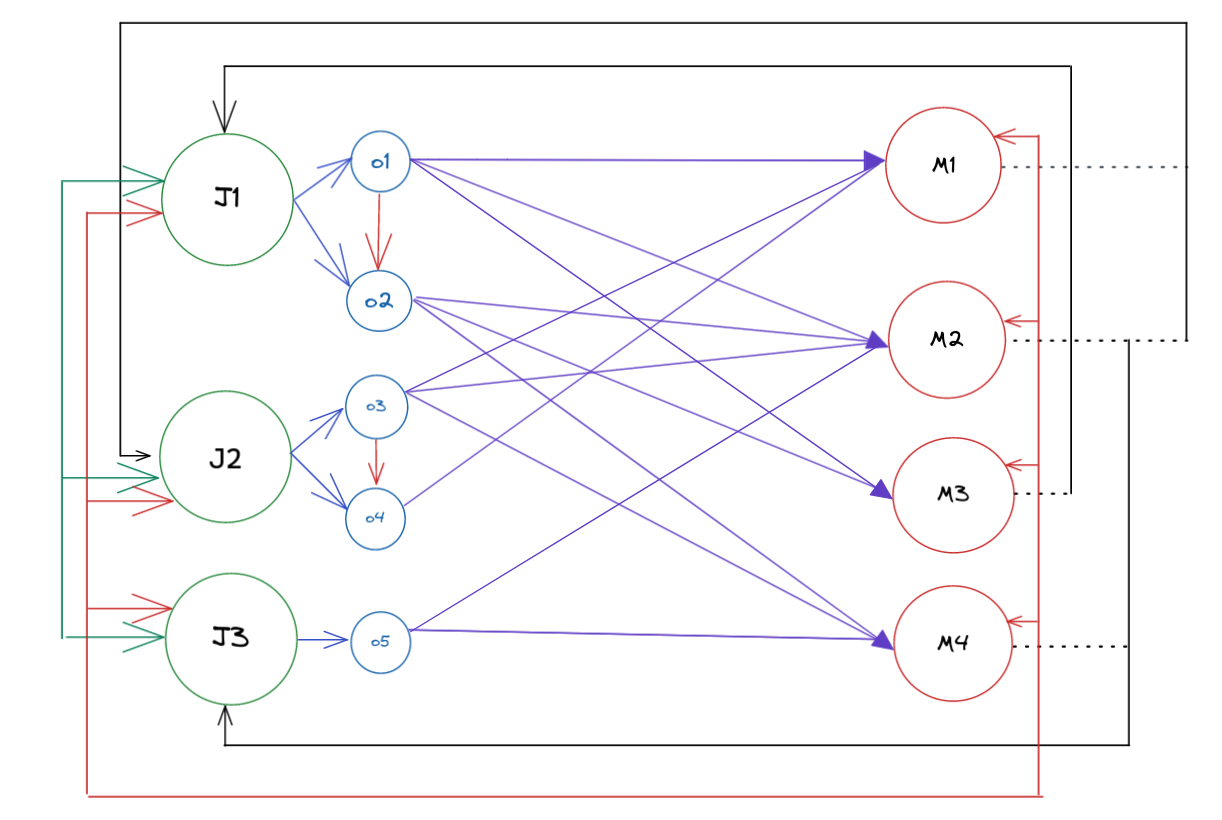
\includegraphics[scale=0.33]{final.png}
    \caption{Estado inicial del la instancia presente en el cuadro 1}
    \label{fig:final-solution}
\end{figure}

\subsubsection{Espacio de acciones}
El espacio de acciones es el conjunto de acciones que puede realizar el agente en cada estado. 
En nuestro caso, se pueden definir el conjunto de acciones como la lista de todas las tuplas 
formadas por las operaciones que pueden ser ejecutadas en cada estado y las máquinas en las que
pueden ser ejecutadas. Por ejemplo, en el estado de la Figura \ref{fig:final-solution} se pueden
definir las siguientes acciones: (Máquina 1, Operación 1), (Máquina 1, Operación 3), 
(Máquina 2, Operación 1), (Máquina 2, Operación 3), (Máquina 2, Operación 3), (Máquina 3, Operación 1), 
(Máquina 4, Operación 5). En este caso, todas aquellas operaciones que no se encuentren en la lista 
de acciones disponibles no pueden ser ejecutadas en el estado actual.

\subsubsection{Transición de estados}
La transición de estado o step es la función que se encarga de actualizar el estado del environment
en base a la acción que ha realizado el agente. En nuestro caso, la función de transición de estados
se encarga de actualizar el grafo con los nuevos tiempos de procesamiento de las operaciones y máquinas, 
así como los gaps existentes entre las operaciones de cada máquina y el resto de atributos de los nodos.\medskip

Para controlar el orden en el que se ejecutan las operaciones y se asignan las máquinas, se ha
decidido utilizar una cola a modo de historial de acciones. De esta forma, cuando el agente realiza
una acción, esta se añade a la cola y se ejecuta la operación que se encuentra en la cabeza del historial
de acciones. El objetivo de este historial no es solo tener un seguimiento del orden de ejecución de las operaciones, sino
que también permite llevar un control mas atómico del environment. De esta forma, si el agente realiza
una acción con lo que no estamos de acuerdo, podemos deshacer la acción y volver al estado anterior
simplemente eliminando la acción de la cabeza del historial. Además, también nos permite cargar o guardar
estados del environment en cualquier momento de la ejecución del algoritmo.\medskip

El estado inicial del environment se carga a partir de un fichero de texto que contiene la información
de la instancia del problema. De esta forma, se genera un primer grafo que contiene toda la información
de la instancia con el historial de acciones vacío. Desde este estado inicial, se ejecutan las
acciones que el agente va seleccionando y se van añadiendo al historial de acciones. Una vez que todas
las operaciones han sido ejecutadas se llega a un estado final.

\begin{figure}[ht]
    \centering
    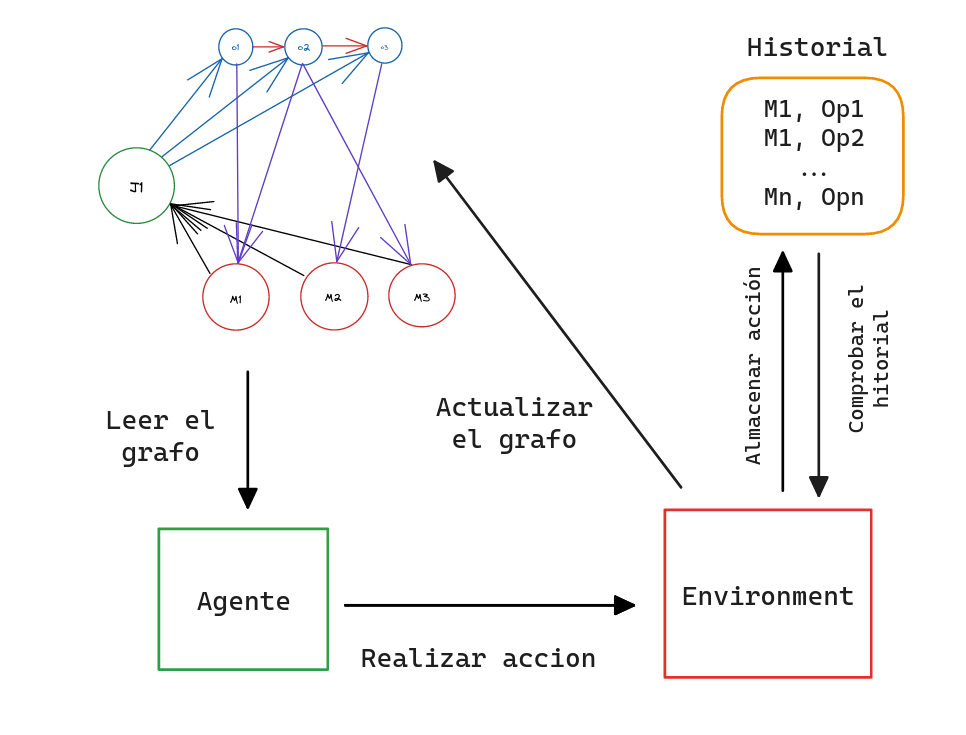
\includegraphics[width=0.9\textwidth]{step.png}
    \caption{Estado inicial del la instancia presente en el cuadro 1}\label{fig:step}
\end{figure}

\pagebreak

\subsection{Generación de instancias aleatorias}
El método de generación de instancias aleatorias se basa en un sistema de instancias sintéticas
que se generan a partir de un conjunto de parámetros de entrada. En el siguiente paper \cite{pbrandimarte}
se define una tabla con diferentes rangos de valores para cada parámetro en cada conjunto de
tamaños de instancias. En nuestro caso, se va a utilizar tres conjuntos de tamaños de instancias
representados en la siguiente tabla.

\begin{table}[ht]
    \centering
    \begin{tabular}[t]{|l|ccc|}
        \hline
                  & Ins. Pequeña & Ins. Medianas & Ins. Grandes \\
        \hline
        Min. num Trabajos    & 3    & 5     & 10    \\
        Max. num Trabajos    & 5    & 10    & 20    \\
        Min. num Operaciones & 2    & 5     & 5     \\
        Max. num Operaciones & 5    & 10    & 10    \\
        Min. num Máquinas    & 2    & 4     & 8     \\
        Max. num Máquinas    & 4    & 8     & 16    \\
        \hline
    \end{tabular}
    \caption{Conjuntos de tamaños de instancias}
\end{table}

En este caso se va a almacenarlas las instancias una vez generadas para poder asegurar la reproducibilidad 
de los resultados, esto adicionalmente implica otros beneficios como el ahorro de tiempo de procesamiento
a la hora de entrar el modelo que se vera altamente beneficiado cuando en pasos posteriores se calcule
las rutas optimas de fabricación de las instancias. Estas conforman nuestro conjunto de datos de 
entrenamiento, de los cuales extraeremos una pequeña parte por cada grupo de instancias para formar
diferentes conjuntos de validación. 

\subsection{Modelos de programación matemática}
Los modelos de programación matemática son una herramienta muy poderosa para resolver problemas
de optimización, en este caso se va a utilizar una librería de código abierto llamada OR-Tools 
\cite{ortools} que esta desarrollada por Google y es utilizada para resolver problemas de optimización 
combinatoria. La librería proporciona algoritmos para resolver una amplia variedad de problemas 
de programación matemática, como problemas de programación lineal, programación entera mixta, 
programación de enteros, y otros problemas de optimización combinatoria.\medskip 

Dentro de la librería se encuentra un modulo llamado \textbf{CP-SAT} que es un modulo de programación
de restricciones que utiliza el algoritmo de búsqueda de satisfacción de restricciones (CS) para resolver
problemas de programación de tareas. Este modulo es el que se va a utilizar para resolver el problema y
dentro de la documentación \cite{ortools-jobshop} de la librería se encuentra un ejemplo de como 
aplicarlo de forma sencilla. La entrada de OR-Tools es una lista de tareas, donde cada tarea contiene
una lista de máquinas que pueden realizar la operación junto con el tiempo de procesamiento.\medskip

\begin{lstlisting}
    jobs_data = [                   
        [(0, 3), (1, 2), (2, 2)],   # Job0
        [(0, 2), (2, 1), (1, 4)],   # Job1
        [(1, 4), (2, 3)]            # Job2
    ]
   
    process_jobs(jobs_data)

    Output:
    Machine 0: [0,3] [3,5]
    Machine 1: [0,4] [4,6] [7,11]
    Machine 2: [5,6] [6,8] [8,11]
\end{lstlisting}

Este resultado muestra una configuración optima de fabricación, de la que se pueden extraer
adicionalmente los tiempos de inicio y fin de cada operación, una representación en forma de
diagrama de Gantt y el make span de la configuración. El make span es el tiempo total que se 
tarda en completar todas las operaciones de la configuración, y es el valor que se va a utilizar
para evaluar la precision de los modelos de deep learning. Con este valor ya seriamos capaces
de conformar los diferentes sets de validación, ya que para esta no es necesario como tal ningún
dato adicional. 

\subsection{Entrenamiento del modelo de deep learning}
\subsubsection{Arquitectura del modelo }
La arquitectura del modelo de deep learning se forma a partir de la combinación de tres 
modelos basados en redes neuronales de grafos que forman un único modelo que es capaz 
de adaptarse a los diferentes tipos de instancias que tenga que predecir. Normalmente en el
ensemble learning se utiliza diferentes técnicas como la votación o la media de los resultados
para elegir las diferentes acciones que se van a tomar, esto es debido a que en ese tipo de problemas
no suele haber una única solución correcta o a que no existe un criterio que permita 
elegir una solución sobre otra. En nuestro caso, debido al claro objetivo que es reducir 
el make span, se va a utilizar la solución que tenga el menor make span de entre las tres 
generadas por los modelos. Los tres modelos que se van a seleccionar son aquellos tres 
que mejor resultado hayan dado en la fase de validación.\medskip

A continuación, se puede ver como esta definido el modelo basado en redes neuronales de grafos.
Para este caso se ha están utilizando capas convolucionales GATv2Conv que son específicas para
el procesamiento de aristas dentro de grafos. Estas capas convolucionales pertenecen a la librería
de Pytorch Geometric \cite{pytorch-geometric} que es una librería de código abierto que proporciona
implementaciones de algoritmos de aprendizaje profundo sobre grafos. 

\begin{figure}[ht]
    \centering
    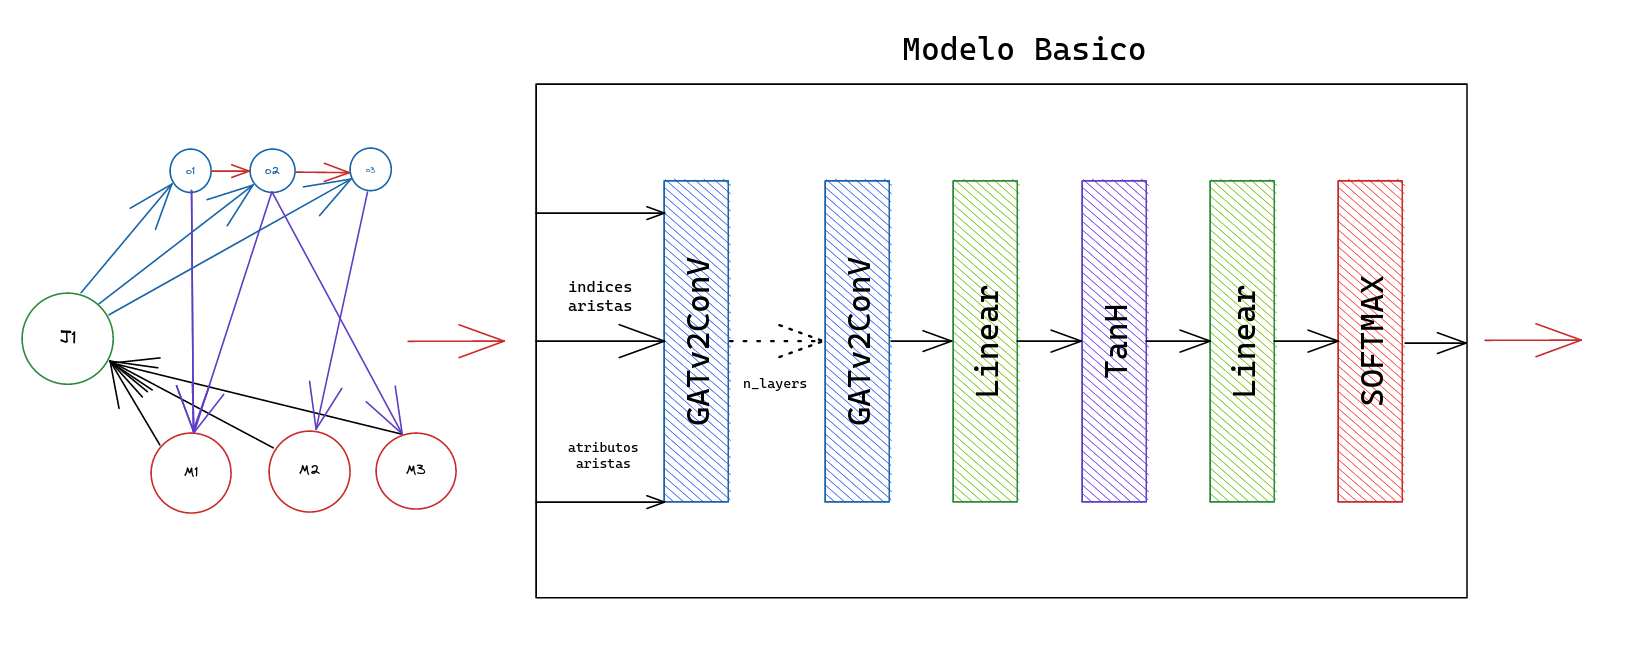
\includegraphics[scale=0.25]{normalmodel.png}
    \caption{Modelo basado en redes neuronales de grafos}
    \label{fig:basicmodel}
\end{figure}

Esta versión del modelo funciona como un agente de RL que recibe como entrada un grafo que representa
un estado del problema, y como salida devuelve la acción que debe tomar para avanzar al siguiente estado.
Para el entrenamiento, utilizaremos esta arquitectura básica ya que es la que mejor
en términos de eficiencia para posteriormente aplicar el ensemble learning.

\subsubsection{Procesado de los datos de entrenamiento}
En la sección anterior se ha visto como se puede obtener una una solución óptima partiendo de una 
instancia del problema, pero para poder entrenar el modelo de deep learning es necesario
que los datos de entrenamiento estén en un formato que sea capaz de procesar el modelo. Para ello,
vamos a conformar un dataset que contenga por un lado un estado del problema y por otro lado la
acción que el experto ha tomado para resolverlo.\medskip

Una de las utilidades de la librería OR-Tools es que el resultado guarda en las operaciones
un atributo que representa en que orden han sido seleccionadas, por lo que es posible mediante 
una simple función de ordenamiento conseguir una sucesión de acciones para llegar a la solución.
Por ultimo, debido a que guardar el grafo directamente en el dataset no es posible debido a que
no es un tipo de dato que se pueda serializar fácilmente, se va a guardar una representación en forma de
matriz de adyacencia del grafo. Esta matriz de adyacencia representara las conexiones de tal modo que 
se pueda cargar y procesar de forma sencilla.

\begin{figure}[ht]
    \centering
    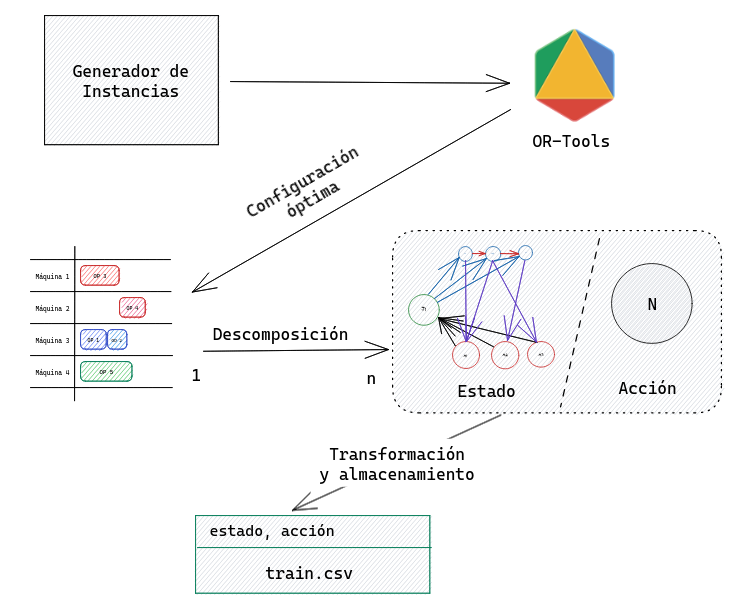
\includegraphics[scale=0.47]{generate_train.png}
    \caption{Pipeline para generar el train.csv}
    \label{fig:trainingpipeline}
\end{figure}

\subsubsection{Funcion de entrenamiento}
Una vez que se ha generado el dataset de entrenamiento, se puede proceder a entrenar el modelo.
Se va a definir una función train que recibe como parámetros el modelo, el optimizador del modelo
de Deep Learning, el dataset
que hemos generado previamente y el tamaño del batch. Esta función se encarga de entrenar el modelo
y devolver el calculo del loss que se ha obtenido durante el entrenamiento.\medskip

\begin{figure}[ht]
\begin{lstlisting}
def train(model, optimizer, train_loader, batch_size):
    model.train()
    softmax = torch.nn.Softmax(dim=0)
    total_examples, total_loss = 0, 0

    for batch in train_loader:
        optimizer.zero_grad()
        action_prob = torch.Tensor([])
        result = model(batch)

        list_action_prob = []
        list_targets = []

        for i in range(batch["job"].batch[-1] + 1):
            action_probs = result[batch_index == i].T[0]
            action_prob = softmax(action_probs)
            list_action_prob.append(action_prob)
            list_targets.append(
                batch[("machine", "exec", "job")].y[batch_index == i]
            )

        loss = F.binary_cross_entropy(list_action_prob, list_targets)
        loss.backward()
        optimizer.step()

        total_examples += batch_size
        total_loss += float(loss) * batch_size

    return total_loss / total_examples 
\end{lstlisting}\medskip
    \caption{Train code example}
    \label{fig:traincode}
\end{figure}

Esta función es la responsable de efectuar el Imitation Learning, para ello carga en el
batch de entrenamiento los grafos que habíamos generado previamente y se le pasa al modelo para que
realice la predicción. Una vez que se tiene la predicción, se calcula el loss y se compara
con la solución que ha tomado el experto para ese estado. Una de las particularidades que
tiene el modelo es que la predicción que devuelve se realiza sobre el tensor que representa
la relación entre las operaciones y las máquinas, por lo que aunque aumente o disminuya 
el numero de operaciones o máquinas no sera necesario modificar el modelo, ya que este 
se adapta a diferentes dimensionalidades.

\subsubsection{Arquitectura del ensemble}
Una vez que se ha entrenado el modelo básico, se puede proceder a montar el ensemble.
Como se ha comentado anteriormente, el ensemble se va a componer de 3 modelos, cada uno
de ellos se va a ejecutar de forma independiente y se va a recuperar la solución que 
mejor desempeño haya tenido. A continuación se muestra la arquitectura del ensemble.

\begin{figure}[ht]
    \centering
    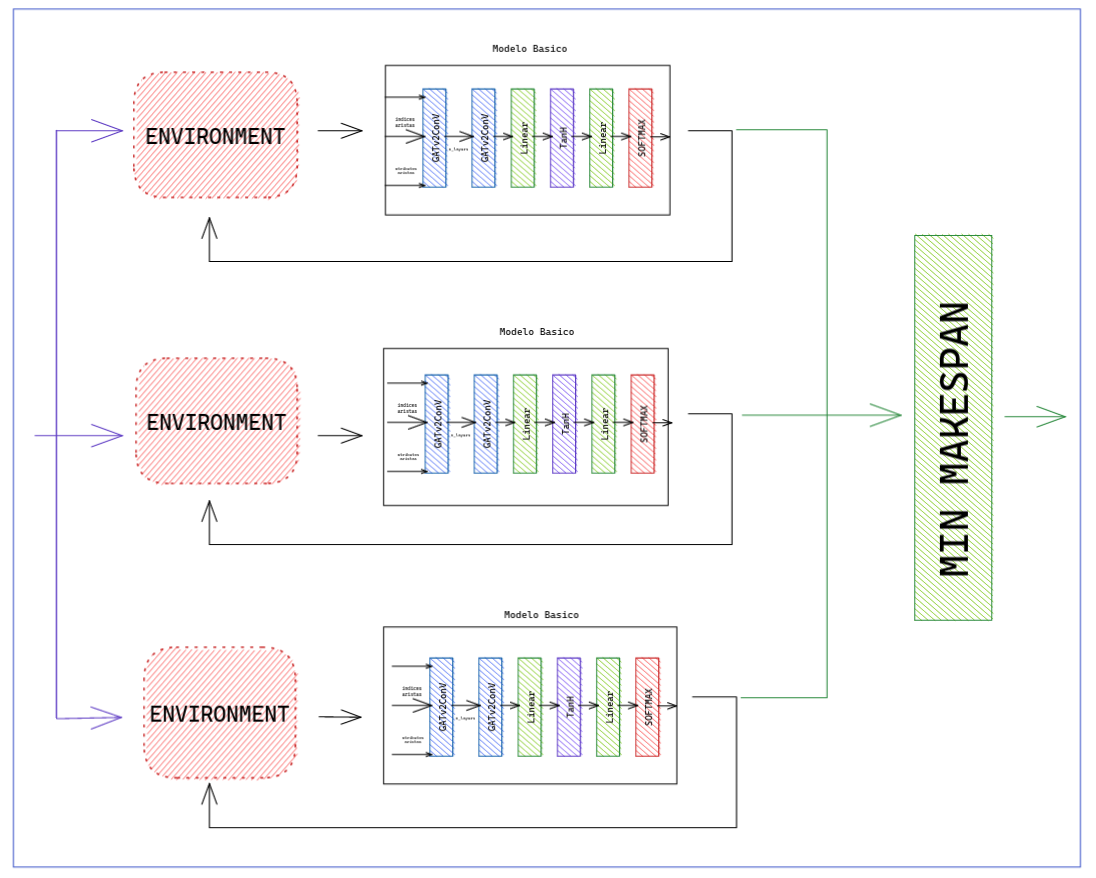
\includegraphics[scale=0.38]{ensemblearc.png}
    \caption{Arquitectura del ensemble}
    \label{fig:ensemblearc}
\end{figure} 

De cara a un futuro, se podría plantear la posibilidad de añadir mas modelos al ensemble
incluso de diferentes tipos entre si. Por ejemplo, se podría añadir un modelo con 
distinto tipo de arquitectura o incluso un modelo que no sea de deep learning. Otra 
posibilidad también seria la de añadir un sistema de votación o stacking para que 
la acción que se tome sea la que mas votos haya obtenido entre los modelos. Se
podría realizar una primera pasada como la que se ha hecho en este trabajo y posteriormente
realizar una segunda pasada mediante un sistema de stacking en la que los pesos de los
modelos se calculen en base a su desempeño en la primera pasada.
\subsection{Modelos de programación matemático}
\subsection{Sistema de evaluación del modelo}
Un buen sistema de evaluación es esencial para un proyecto de Machine Learning.
No solo es útil por el hecho de medir el rendimiento de los modelos,
sino que además sirve como un identificador claro del progreso dentro del desarrollo.
El seleccionar el modelo óptimo en fases tempranas del proceso no es tan importante,
como el hecho de saber que las iteraciones en las que gastamos tiempo y recursos están teniendo un impacto
positivo en el resultado final. Aunque físicamente es imposible conseguir una productividad
perfecta, con ayuda de una metodología sólida es posible reducir al máximo esta problemática.

\subsubsection{Selección de métrica}
El objetivo de una métrica es, mediante ponderación numérica, identificar errores en el modelo y
servir como ayuda para la toma de decisiones, cambios en el diseñe o la solución de problemas. En el caso del
FJSP, el objetivo es encontrar una acorde a la tarea que queramos abordar. En la literatura se atacan dos puntos
principalmente: \textit{minimizar el tiempo de finalización} y \textit{minimizar el tiempo de espera entre máquinas}.

\begin{itemize}
    \item \textbf{Minimizar el tiempo de espera entre máquinas:} mide el tiempo promedio que cada operación debe
          esperar antes de ser procesado en una máquina específica. Esta métrica es importante porque
          indica la eficiencia del sistema en términos de cómo se están utilizando los recursos disponibles
          y cómo se gestionan los trabajos en las colas.
    \item \textbf{Minimizar el tiempo de finalización:} se basa en el tiempo total que se tarda en completar todos
          los trabajos del sistema. Es un buen indicador porque evalúa el rendimiento global del sistema
          y la eficacia para completar el proceso en el plazo establecido.
\end{itemize}

Aunque ambas métricas son importantes, la segunda es la que vamos a utilizar como referencia en cuanto al
desempeño del modelo se refiere, ya que uno de nuestros objetivos principales es reducir los tiempos de producción y no tanto
aprovechar las máquinas lo máximo posible. Es una opción combinar ambas para identificar puntos débiles tanto del modelo
como del propio proceso que se quiere optimizar pero, por la propia idiosincrasia de estas métricas, el mejorar la puntuación
en una inevitablemente afectara negativamente a la valoración de la otra en un amplio número de casuísticas.

\subsubsection{Implementación de la métrica}
Ya hemos decidido que métrica es la indicada para evaluar nuestro modelo, pero ahora debemos
implementarla de acorde al contexto de nuestro problema. El siguiente paper utiliza una formula para
calcular el time spam que nosotros también vamos a utilizar, donde Tmax es el tiempo que tarda en
finalizar el sistema y Tmin el tiempo óptimo de finalización. Nuestro objetivo como hemos mencionado
previamente es acercarnos lo máximo posible a la combinación optima, que en este caso seria lo equivalente a
aproximarnos lo más que podamos al 0. Además, gracias a que nuestra implementación se basa en una función
matemática, podremos extrapolarla en el apartado de \textit{Benchmarking} no solo a la evaluación de nuestro
modelo, sino también a cualquier otro sistema externo que resuelva el problema.

\medskip
\equationNote{f(x) = \frac{Tmax - Tmin}{Tmin}}{}

\subsubsection{Benchmarking}
Por último, es hora de definir como vamos a realizar el proceso de benchmarking. Hemos comentado en
el apartado anterior, que no solo incluiremos el histórico de las diferentes versiones de nuestro
modelo, sino que también añadiremos otras alternativas para la resolución del problemas como reglas de
ordenación, algoritmos genéticos o métodos exactos. Para ello, contamos con un benchmark de 10 instancias
llamada Brandimarte \cite*{pbrandimarte}, que son las populares dentro de la literatura para la comparación de modelos.
Estas se pueden encontrar en el siguiente repositorio \cite*{ptal} de GitHub.\medskip

\begin{table}[ht]
    \centering
    \begin{tabular}[ht]{c|ccccc|c} 
                  & njob & nmac & nop & meq & proc & optim \\
        \hline 
        MK01      & 10  & 06    & 05 -- 07  & 3  & 01 -- 07  & 40\\
        MK02      & 10  & 06    & 05 -- 07  & 6  & 01 -- 07  & 26\\
        MK03      & 15  & 08    & 10 -- 10  & 5  & 01 -- 20  & 204\\
        MK04      & 15  & 08    & 03 -- 10  & 3  & 01 -- 10  & 60\\
        MK05      & 15  & 04    & 05 -- 10  & 2  & 05 -- 10  & 172\\
        MK06      & 10  & 15    & 15 -- 15  & 5  & 01 -- 10  & 57\\
        MK07      & 20  & 05    & 05 -- 05  & 5  & 01 -- 20  & 139\\
        MK08      & 20  & 10    & 10 -- 05  & 2  & 05 -- 20  & 523\\
        MK09      & 20  & 10    & 10 -- 15  & 5  & 05 -- 20  & 307\\
        MK10      & 20  & 15    & 10 -- 15  & 5  & 05 -- 20  & 196\\
    \end{tabular}
    \caption{Informacion del benchmark}
\end{table}

En la tabla anterior, podemos observar las diferentes características de cada instancia. A continuación,
vamos a explicar cada una de ellas:
\begin{itemize}
    \item \textbf{njob:} Número de trabajos.
    \item \textbf{nmac:} Número de máquinas.
    \item \textbf{nop:} Número mínimo y máximo de operaciones por trajo.
    \item \textbf{meq:} Número máximo de máquinas equivalentes por operación.
    \item \textbf{proc:} Número mínimo y máximo de tiempo de procesamiento por operación.
    \item \textbf{optim:} Valor óptimo para la resolución.
\end{itemize} 

Además, el paper \cite*{pbrandimarte} también incluye una tabla con los resultados de diferentes
reglas de ordenación y otra clase de algoritmos como la búsqueda tabú. Esto nos sera de gran ayuda
para comparar nuestro modelo con otros y ver si realmente estamos mejorando los tiempos en
comparación con otras alternativas, no solo en el caso de que nuestro modelo sea mejor, sino también
en el caso de que no lo sea. En este último caso, podremos analizar los resultados y ver si es posible
realizar cambios en el enfoque del problema para mejorar los resultados.

\pagebreak
    \section{Experimentacion y resultados}
    \section{Conclusiones y trabajo a futuro}
    \section{Definiciones, Acrónimos y Abreviaturas}
\subsection{Acrónimos y Abreviaturas}
\begin{itemize}
    \item \textbf{FJSP: } Flexible Job Shop Scheduling Problem.
    \item \textbf{JSP: } Job Scheduling Problem.
    \item \textbf{IA: } Inteligencia Artificial.
    \item \textbf{RL: } Reinforcement Learning.
    \item \textbf{IL: } Imitation Learning.
    \item \textbf{CSV: } Comma Separated Values.
\end{itemize}

\subsection{Definiciones}
\begin{itemize}
    \item \textbf{Linter: } Un linter es una herramienta que analiza el código fuente 
    para señalar errores de programación, errores de estilo, construcciones sospechosas, etc.
    \item \textbf{Formateador: } Un formateador es una herramienta que analiza el código fuente
    para formatearlo de forma que cumpla con un estilo de código concreto.
    \item \textbf{Modelo: } Un modelo de ML es un algoritmo que aprende de los datos
    para realizar una tarea específica. 
    \item \textbf{Environment: } Un environment es un entorno donde se ejecuta un agente
    de RL. El environment proporciona al agente información sobre el estado del entorno
    y el agente puede realizar acciones que afectan al environment.
\end{itemize}

\pagebreak 
    \printbibliography[title=Bibliografía]

\end{document}